%%%%%%%% ICML 2027 submission: Weak and Strong Compositionality %%%%%%%%
% Built from ../recoverability-theory/main.tex (the long preprint). The main body is condensed to the
% 8-page limit; parts/*.tex hold the long sections, moved verbatim into the appendix.
\documentclass{article}

\usepackage[T1]{fontenc} % Tectonic (XeTeX) defaults to TU, which has no Times; T1 gives the Type-1 Times of icml2027.sty
\usepackage{microtype}
\usepackage{graphicx}
\usepackage{booktabs}
\usepackage{tabularx}
\usepackage{hyperref}
\newcommand{\theHalgorithm}{\arabic{algorithm}}

% Initial blind submission:
\usepackage{icml2027}
% Preprint: \usepackage[preprint]{icml2027}
% Camera-ready: \usepackage[accepted]{icml2027}

\usepackage{amsmath,amssymb,mathtools,amsthm}
\usepackage{enumitem}
\usepackage{placeins}
\usepackage[most]{tcolorbox}

\definecolor{refnavy}{HTML}{001473}
\definecolor{boxframe}{HTML}{B2D9D9}
\definecolor{boxfill}{HTML}{F7FBFB}
\hypersetup{colorlinks=true,linkcolor=refnavy,citecolor=refnavy,urlcolor=refnavy}
\graphicspath{{figures/}}

% Tinted boxes for the formal definitions (as in the preprint).
\tcbset{recbox/.style={enhanced, colback=boxfill, colframe=boxframe, boxrule=0.6pt,
  sharp corners, left=4pt, right=4pt, top=3pt, bottom=3pt, fonttitle=\bfseries, coltitle=black,
  attach title to upper, after title={.\ }, separator sign={.}, description delimiters none,
  description font=\bfseries}}
\newtcbtheorem{defbox}{Definition}{recbox}{def}

\theoremstyle{plain}
\newtheorem{proposition}{Proposition}
\newtheorem{observation}[proposition]{Observation}
\newtheorem{lemma}{Lemma}
\theoremstyle{remark}
\newtheorem*{remark}{Remark}
\newcommand{\R}{\mathbb{R}}
\newcommand{\U}{\mathcal{U}}
\newcommand{\M}{\mathcal{M}}
\newcommand{\D}{\mathcal{D}}
\newcommand{\Voc}{\mathcal{V}}
\newcolumntype{Y}{>{\raggedright\arraybackslash}X}
\newcolumntype{P}[1]{>{\raggedright\arraybackslash}p{#1}}
\setlist{itemsep=1pt,topsep=3pt,parsep=0pt}

\icmltitlerunning{Weak and Strong Compositionality}

\begin{document}

\twocolumn[
  \icmltitle{Benchmarks Test Weak Compositionality, but Strong Compositionality Needs Decomposition}

  % Author information is removed automatically unless [accepted] is passed.
  \begin{icmlauthorlist}
    \icmlauthor{Karthik Singaravadivelan}{gt}
  \end{icmlauthorlist}
  \icmlaffiliation{gt}{College of Computing, Georgia Institute of Technology, Atlanta, GA, USA}
  \icmlcorrespondingauthor{Karthik Singaravadivelan}{ANONYMIZED}

  \icmlkeywords{compositionality, systematicity, decomposition, representation, probing, ICML}

  \vskip 0.3in
]

\printAffiliationsAndNotice{}

\begin{abstract}
Anyone who can think that John loves Mary can also think that Mary loves John, yet benchmarks of compositionality in neural networks score only whether a model acts correctly on new combinations of known parts, a test that a lookup table passes. We separate weak compositionality, which recombines known parts, from strong compositionality, which also builds wholes that come apart again, and we measure this decomposition by recoverability, a calibrated score of how well a linear probe, fixed in advance, returns parts new to it. We hypothesize that behavioral compositionality is a subset of representational compositionality, able to do some, and not all, of the things representational compositionality can do. In toy networks, and in image encoders and diffusion models at fixed places, states keep parts that the system's own outputs lose, and procedures that read the toy states repair the behavior. Test-time harnesses repair answers and image layouts where their code, or a model that answers by meaning, assigns the roles. Every pretrained state we tested binds roles to position, by order of mention in sentences and by absolute place in images, and a role by meaning appears only at the question, in language models that answer by meaning. Every family of behavioral tests in current use scores the weak form, and we close with the components of a benchmark for the strong one.
\end{abstract}

%=====================================================================
\section{Introduction}
\label{sec:intro}

Composition is the study of parts and their combination through some operation. A compositional system builds wholes from reusable parts, so that the meaning of a sentence follows from the meanings of its words and the way they combine \citep{frege1923,janssen1997}. People understand sentences they have never heard \citep{chomsky1957}, a person who learns the verb \emph{dax} understands \emph{dax twice} at once \citep{lake2018}, and anyone who can think that John loves Mary can think that Mary loves John \citep{fodor1988}. A compositional system handles new combinations of known parts, and it can also use a new part in every role, add knowledge without damaging old knowledge, nest wholes inside wholes and keep each part in its role \citep{lake2017}.

Wholes differ in how much of their parts they keep (Appendix Figure~\ref{fig:intro}). Two photographs side by side keep both pictures and their places, while $x + y$ loses the order of its parts, because it equals $y + x$. We call the building of a whole \emph{composition}, and the return of the same parts in the same roles \emph{decomposition}.

Current tests score composition through behavior. Benchmarks ask a model to act on new combinations of training parts \citep{lake2018,keysers2020,hupkes2020}, vision--language benchmarks swap the roles in a caption \citep{thrush2022winoground,yuksekgonul2023}, detectors judge the scenes that text-to-image models compose \citep{ramesh2021,huang2023t2i}, and reasoning tests chain facts that a language model knows one at a time \citep{press2023}. A lookup over a finite vocabulary passes these tests (Section~\ref{sec:definition}).

\begin{figure*}[t]
  \centering
  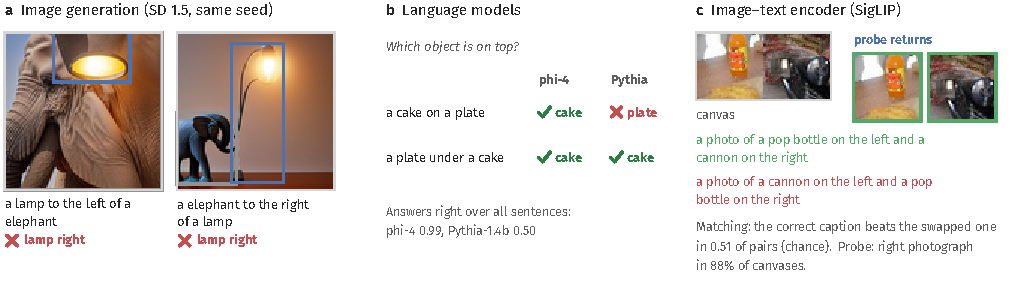
\includegraphics[width=0.92\textwidth,trim=0 0.22in 0 0,clip]{fig_case_motivate.pdf}
  \caption{\textbf{One relation in two orders.} \textbf{a.} Under one seed, SD 1.5 draws the same layout for a prompt and its converse, with the lamp on the wrong side both times (prompts verbatim; the first gallery pair of Appendix Figure~\ref{fig:case_generation} whose phrasings share a layout and misplace the figure). \textbf{b.} phi-4 answers by meaning, and Pythia-1.4b names the second-mentioned noun. \textbf{c.} SigLIP prefers the correct caption over the place-swapped one on 0.51 of pairs, while a linear probe of its quadrant states returns the right photograph for 88\% of canvases.}
  \label{fig:motivate}
\end{figure*}

Consider one relation stated in two orders (Figure~\ref{fig:motivate}). Asked for a lamp to the left of an elephant and for the converse phrasing, Stable Diffusion 1.5 draws the same scene under the same seed, so the relation word leaves the layout in place. Asked which object is on top in ``a cake on a plate'' and in ``a plate under a cake'', phi-4 answers \emph{cake} twice, while Pythia-1.4b answers \emph{plate} and then \emph{cake}. SigLIP matches a canvas to the caption with the places swapped as often as to the correct one, yet a linear probe of its patch states returns both photographs in their places. A behavioral test cannot say whether a failing system lost the parts or merely failed to read them \citep{conwell2022,rassin2022}.

We propose that compositionality is a spectrum of capabilities with two forms, one containing the other. \emph{Weak compositionality} combines known parts into new wholes and acts on them correctly, and \emph{strong compositionality} also builds wholes that come apart again.

The two notions form a weak and a strong version of composition. Behavioral compositionality is the weak version, in which a system composes parts, and any decomposition it performs comes from a procedure trained for that purpose. Representational compositionality is the strong version, in which a system composes parts and its composites also decompose. Recoverability is our heuristic for the strong version, and it asks whether parts read out easily from the internal states of a composite. Decomposition matters because it supports the efficient use of parts and reveals what each part donates to the whole.

Decomposition needs a careful test, because a lookup table over the training parts takes apart any whole that keeps them distinct, and a flexible enough probe decodes almost anything \citep{hewitt2019}. Our probe is therefore linear and fixed before we see any result, and it must succeed on parts it never saw in its own training. Recoverability scores decomposition under both demands, from 0 for the sum of the parts to 1 for a side-by-side copy of each.

We hypothesize that behavioral compositionality is a subset of representational compositionality, able to do some, and not all, of the things representational compositionality can do. A model whose own procedure handles new parts must have a state that holds them (Observation~\ref{prop:subset}), while a state can hold parts that the model's outputs miss, and the strictness of the inclusion is the empirical hypothesis that we test.

\begin{figure}[t]
  \centering
  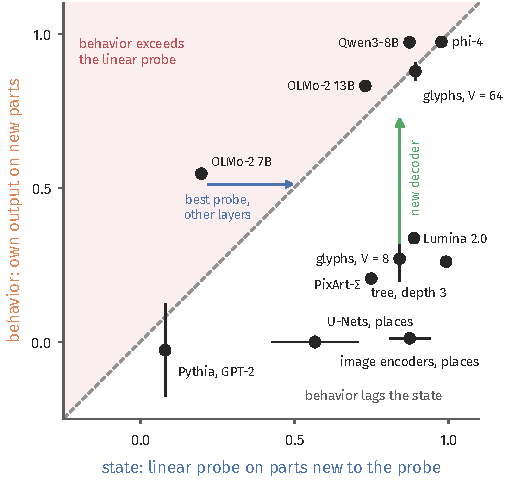
\includegraphics[width=0.92\columnwidth]{fig_ladder.pdf}
  \caption{\textbf{Behavior lags the decomposition that the state supports.} Each system is scored on parts new to the probe, by a linear probe of its state (horizontal) and by its own output (vertical), from a blend, chance or word order (0) to exact recovery (1). Image and diffusion points use fixed quadrants, and open circles move the photographs. A new decoder lifts glyph behavior (green).}
  \label{fig:ladder}
\end{figure}

The evidence favors a strict inclusion. Networks trained on eight glyphs fail to draw new glyphs that a linear probe of their state recovers (Figure~\ref{fig:ladder}). Pretrained systems bind roles to position, by order of mention in sentences and by absolute place in images. Their states pass our test where position and meaning coincide, and they fall short once a converse paraphrase or a moved scene separates the two.

\textbf{Contributions.} (i) A definition of weak and strong compositionality by the capabilities each supports. (ii) A test of decomposition, recoverability $\kappa$, with proofs that tests on training parts cannot detect decomposition and that rank, width and depth each cap it. (iii) Evidence from toy networks to language models with 15 billion parameters that states keep parts that behavior loses. (iv) A diagnosis of positional binding, with each system placed as a pair, test-time harnesses included. (v) A spectrum of twenty-two accounts of compositionality, and (vi) the components of a benchmark for the strong form.

%=====================================================================
\section{Related Work}
\label{sec:related}

\textbf{Meaning and constituents.} Montague made Frege's principle a homomorphism from syntax to semantics \citep{frege1923,montague1970}, yet a recoding of the parts makes any assignment of meanings compositional \citep{zadrozny1994}. \citet{fodor1988} traced systematicity to constituents that appear in every whole that contains them, \citet{smolensky1990} answered with tensor-product representations, and \citet{fodor1990} replied that such implicit constituents cannot act in processing.

\textbf{Tests and measures.} Benchmarks score outputs on new combinations of training parts \citep{lake2018,keysers2020,hupkes2020}. Probes decode constituents from states \citep{belinkov2022}, interventions and tensor-product decompositions supply part vectors \citep{geiger2021,mccoy2019}, and decodable factors need not yield a decoder that generalizes \citep{montero2021}. Compression measures run from parts to whole on the data themselves \citep{andreas2019,elmoznino2024}, and ours runs from whole to parts through a probe fixed in advance on parts new to it. Appendix~\ref{app:related} gives a longer account.

%=====================================================================
\section{Weak and Strong Compositionality}
\label{sec:definition}

\textbf{Parts, wholes and roles.} A part is a draw from a distribution $\D$ over possible parts, such as glyphs, nouns or photographs. A system gives each part $x$ a \emph{part vector} $e(x) \in \R^d$, and it gives a whole $r(x_1, \ldots, x_k)$, built from $k$ parts in the roles of a relation $r$, a state $h = g_r(x_1, \ldots, x_k) \in \R^m$. Training exposes the system to a finite \emph{vocabulary} $\Voc$ of \emph{training} parts. A part is \emph{new to a procedure} when no whole containing it helped fit that procedure. A glyph can be new to both a probe and the network that encodes it, whereas a noun can be new only to the probe of a pretrained model.

Suppose a system adds two part vectors $x$ and $y$. Every pair on the line $x + y = z$ yields the same whole, so no procedure can return the parts. A tensor-product binding $x \otimes \rho_1 + y \otimes \rho_2$ with independent role vectors \citep{smolensky1990} instead keeps one decomposition for each whole. A small vocabulary hides the difference, because few vocabulary pairs share a line and a lookup finds the summed parts, and a new pair exposes it.

\begin{defbox}{Weak compositionality}{behcomp}
A system is \emph{weakly compositional} with respect to a relation $r$ to the degree that its own procedures, such as a decoder, a decomposer or the answering of questions about the roles, give the correct output for new wholes built from training parts.
\end{defbox}

Weak compositionality asks nothing of the way back from a whole to its parts. A relation that loses information can still keep a finite vocabulary distinct, and a lookup table then inverts it (Lemma~\ref{lem:lookup}). A linear procedure fitted on wholes determines its output only on the span of the part vectors those wholes contain, so it reaches new parts only when the training parts in each role span all $d$ dimensions (Proposition~\ref{prop:span}), which restates the argument of \citet{marcus1998} for procedures.

The harder capabilities start from a whole and need its parts back: taking in new parts, placing a new part in every role, adding parts without forgetting, nesting wholes inside wholes and inspecting each part's share (Appendix Table~\ref{tab:capabilities}). Decomposition alone, however, comes cheap. A lookup table and a flexible enough probe both decode almost any whole \citep{hewitt2019}, so we add two conditions.

\begin{defbox}{Decomposition and strong compositionality}{decomp}
The wholes of a relation $r$ \emph{decompose} under a kind of probe $\U$, fixed in advance, if for every role $i$ one probe $u_i \in \U$, fitted on wholes built from some parts, returns the part in role $i$ from wholes built from parts new to it. The relation's meaning fixes its roles; for sentences, role 1 is the figure in either phrasing. A system is \emph{strongly compositional} with respect to $r$ when the states it builds for wholes of $r$ decompose.
\end{defbox}

\textbf{Roles by position and roles by meaning.} Recoverability depends on a declared role assignment, just as it depends on the declared part vector. A probe that returns parts by position, the order of mention in a sentence or a fixed place on a canvas, reads a \emph{positional binding}. Positional binding meets Definition~\ref{def:decomp} only where position and meaning coincide, so our tests of the strong form also move the position and keep the meaning, through converse paraphrases and moved photographs. We report each placement as a pair: the role assignment, and the set the system reaches under it.

\textbf{Behavior and representation.} A state that decomposes supports every weak capability, because a procedure that starts from the returned parts can act on any new combination. The system exhibits a capability only when its own procedure is such a procedure. Conversely, a procedure that returns the parts of wholes built from new parts is itself a probe that succeeds on them, so behavior is included in representation for every kind of probe that contains the procedure (Observation~\ref{prop:subset}). A linear probe need not contain the procedure, so behavior can outrun it, and we report each such case as a limit of the probe.

%=====================================================================
\section{Measuring Decomposition}
\label{sec:repcomp}

A \emph{kind of probe} $\U$ contains the procedures that may recover a part's vector from a state. Throughout the paper the probe is linear, with a bias term. We fix it in advance because, with unrestricted coordinates, every invertible relation becomes additive (Lemma~\ref{lem:psi}), and every system would pass.

\begin{defbox}{Recoverable relations}{recoverable}
Fix a part distribution $\D$, a part vector $e$ and a kind of probe $\U$. A relation $r$, which a system realizes by $g_r$, is \emph{$\varepsilon$-recoverable} if for every role $i$ some $u_i \in \U$ satisfies, for parts drawn independently from $\D$,
\begin{equation}
  \frac{\mathbb{E}\,\lVert u_i(g_r(x_1,\ldots,x_k)) - e(x_i) \rVert^2}{\mathbb{E}\,\lVert e(x) - \mathbb{E}\,e(x) \rVert^2} \;\le\; \varepsilon .
  \label{eq:recover}
\end{equation}
We fit $u_i$ on wholes built from the \emph{probe's training parts} and evaluate it on wholes built from other parts.
\end{defbox}

The quantity $1 - \varepsilon$ is the $R^2$ of the best probe. A symmetric blend already scores $R^2 = 1/2$, because the probe can return the average of the two parts, so we place each system between two references built from the same part vectors.

\begin{defbox}{Recoverability}{repcomp}
A system's \emph{recoverability} for a relation $r$ is
\begin{equation}
  \kappa = \frac{\varepsilon_{\mathrm{blend}} - \varepsilon}{\varepsilon_{\mathrm{blend}} - \varepsilon_{\mathrm{ref}}},
  \label{eq:kappa}
\end{equation}
where the same probe, fitted and tested in the same way, gives $\varepsilon_{\mathrm{ref}}$ for the concatenation and $\varepsilon_{\mathrm{blend}}$ for the sum of the same part vectors. The system is \emph{representationally compositional} at tolerance $\tau$ if $\kappa \ge 1 - \tau$ for a part vector that carries information about the parts (Appendix~\ref{app:defs}).
\end{defbox}

A system scores $\kappa = 1$ when its state gives the parts back as well as laying them side by side would, and $\kappa = 0$ when it gives them back no better than adding them. Every score depends on the part vector that its protocol declares (Appendix~\ref{app:defs}).

\textbf{Shared role codes.}\label{sec:mechanics} The simplest route to recoverability gives each part one vector that enters every whole and changes only with its role.

\begin{defbox}{Shared role codes}{factor}
A relation $r$ has \emph{shared role codes} with residual $\delta$ if, for some vector $e'$ of which $e$ is a linear function, some $c \in \R^m$ and injective matrices $B_1, \ldots, B_k$, one per role and shared by all parts,
\begin{equation}
  g_r(x_1, \ldots, x_k) = c + \textstyle\sum_{i} B_i\, e'(x_i) + \eta,
  \label{eq:factor}
\end{equation}
with $\mathbb{E}\,\lVert \eta \rVert^2 \le \delta\, \mathbb{E}\,\lVert g_r - \mathbb{E}\,g_r \rVert^2$.
\end{defbox}

Shared role codes formalize the classical demand that a constituent contribute the same thing to every complex that contains it \citep{fodor1988}, and a tensor product with independent roles meets it with $\delta = 0$ \citep{smolensky1990}. With full-rank role maps, one whole fixes every role reversal and every assignment of a known part to a new role (Propositions~\ref{prop:systematic} and~\ref{prop:approx}). Three limits follow from the definitions. A linear blend loses a computable share of its parts, half of each part for $x + y$ (Proposition~\ref{prop:ceiling}). A state of width $m$ caps any linear probe at the share of the parts' variance in their top $m$ principal components (Proposition~\ref{prop:ey}). Nesting a blend $n$ levels deep loses at least $(2^n - 1)d$ dimensions of its leaves unless the state grows with depth (Proposition~\ref{prop:depth}).

\textbf{Tests on training parts cannot see decomposition.} On fourteen toy operators of two Gaussian parts, a lookup over 32 training parts identifies the role-1 part with accuracy 1.00 for every operator that keeps the vocabulary distinct, including holographic reduced representations (HRR) that keep half of each part. On new parts, linear probes meet the ceilings, with $R^2 = 1.00$ for role--filler binding, 0.80 for $x + 0.5y$ and 0.44 for HRR, while an MLP probe memorizes the vocabulary (Appendix~\ref{app:calibration}).

%=====================================================================
\section{Experimental Setup}
\label{sec:experiments}

We test four hypotheses on parts new to every fitted procedure. \textbf{H1}: where a system's own procedure acts correctly on new parts, a probe of the state it reads recovers them. \textbf{H2}: behavior can lag the state. \textbf{H3}: a procedure that reads a recoverable state lifts behavior. \textbf{H4}: a state owes its recoverability to its input, its architecture or its training.

\textbf{Systems.} \emph{Glyph networks} (MLP, CNN, transformer and role--filler encoders with decoders) encode two $8 \times 8$ glyphs on a canvas under three relations, trained on vocabularies of $V = 8$ to 64 glyphs, so a glyph can be new to the network itself. \emph{Recursive composers} \citep{pollack1990} compose trees of Gaussian leaves, trained on depths 1 and 2. \emph{Image encoders} (CLIP B/32 and H/14, DINOv2, SigLIP) and \emph{diffusion models} (SD 1.5 and SDXL) read two Tiny-ImageNet photographs on one canvas \citep{radford2021clip,cherti2023,oquab2024dinov2,zhai2023siglip,rombach2022,le2015tiny}. \emph{Language models} (phi-4, Qwen3-8B, OLMo-2 7B and 13B, seven Pythia models, GPT-2) and eleven text encoders read sentences such as ``a $x$ on a $y$'' over 305 concrete nouns in five asymmetric relations \citep{abdin2024phi4,yang2025qwen3,olmo2024olmo2,biderman2023pythia,radford2019gpt2}. In pretrained models parts are new only to the probe, apart from invented words, and Appendix~\ref{app:setup} lists every system.

\textbf{Roles by meaning.} Each relation has a \emph{converse} paraphrase that reverses the order of mention while keeping the meaning, as in ``a tulip on a barrel'' and ``a barrel under a tulip''. The tulip is the \emph{figure} in both, and the barrel is the \emph{ground}. Language models answer ``Which object is on top?'' after four demonstrations, and we call the state at the final token the \emph{question state}. Image--text encoders match a canvas against a caption and against the same caption with the places swapped.

\textbf{Protocol and metrics.} We split the parts before we fit anything, and new parts give every reported number. For a pretrained model, a part vector is the model's state for one part alone, reduced to 16 whitened principal components \citep{timkey2021}, and validation parts choose only the ridge penalty, the layer and the part vector. Each system also runs with random weights. We report recovery $R^2$, recoverability $\kappa$, \emph{role transfer} (the share of converse sentences on which a figure probe fitted on canonical sentences lands nearer the figure than the ground, so word order scores 0), answer accuracy (word order scores 0.5), the flip rate of answers under activation patches, and the role residual $\delta$. Appendices~\ref{app:setup} and~\ref{app:protocol} give the details.

%=====================================================================
\section{Results}
\label{sec:results}

\begin{figure*}[t]
  \centering
  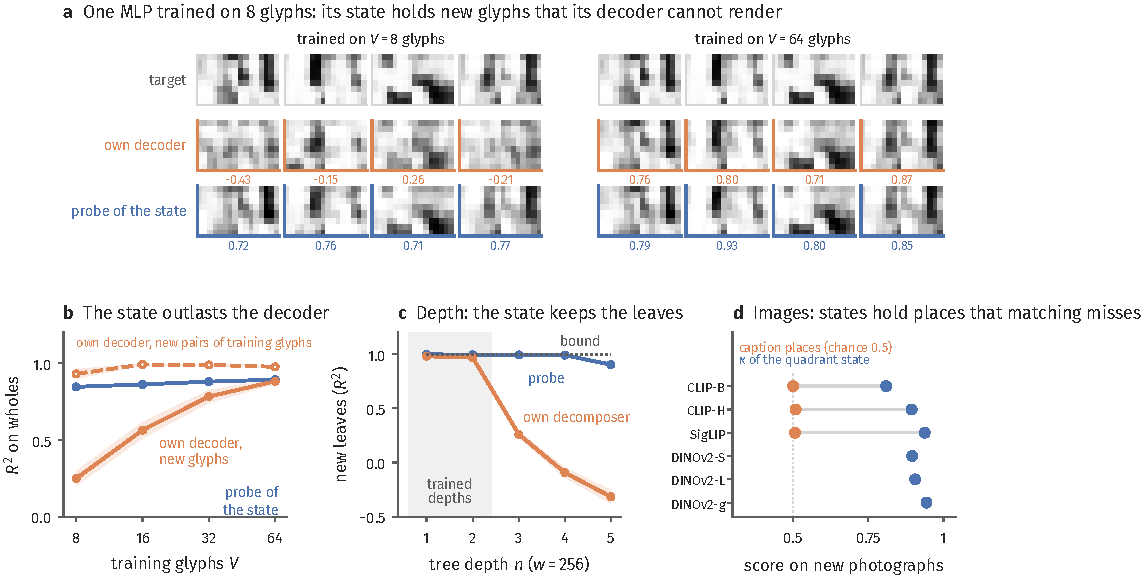
\includegraphics[width=0.80\textwidth]{fig_strong_only.pdf}
  \caption{\textbf{States decompose where the system's own outputs stay weak.} \textbf{a.} Trained on 8 glyphs, an MLP renders new glyphs poorly (orange), while a linear probe of its state recovers them (blue); trained on 64, it does both. Numbers give $R^2$ to the target. \textbf{b.} Own decoders reproduce new pairs of training glyphs (dashed, open) and fail on new glyphs at small $V$ (solid), while the probe stays high ($m = 64$). \textbf{c.} A recursive composer's decomposer fails beyond its training depths (shaded), while a probe of the root state follows the bound of Proposition~\ref{prop:depth} (dotted). \textbf{d.} Image--text encoders match swapped-place captions at chance, while their quadrant states recover both photographs. Means over 3--9 seeds, with standard errors.}
  \label{fig:strong}
\end{figure*}

\subsection{Glyph Networks Keep New Glyphs Their Decoders Cannot Draw}
\label{sec:states}

Every architecture reproduces new pairs of training glyphs with output $R^2$ of 0.85--1.00, apart from the transformer at $V = 8$. New glyphs are harder: output $R^2$ rises from 0.20--0.34 at $V = 8$ to 0.85--0.91 at $V = 64$ (Figure~\ref{fig:strong}b). The states keep the new glyphs throughout. At $V = 8$, a broad probe of the MLP, CNN and role--filler states recovers 0.83--0.86, while a probe fitted only on the training glyphs recovers 0.23--0.29 and tracks the network's own output, as Proposition~\ref{prop:span} predicts. A new decoder trained on the frozen encoder renders new glyphs at 0.75, against 0.25 for the network's own decoder (Appendix Figure~\ref{fig:case_glyph}).

The decoders also read the role codes. Under \textsc{over}, the role residual is $\delta = 0.02$--$0.04$. Writing a donor's vector into role 1 makes the decoder render the donor at $R^2 = 0.78$ and spills only 0.16 into the untouched half, so the constituents act in processing, as \citet{fodor1990} demanded. Written vectors also add 32 glyphs in sequence and keep old pairs at 0.99, where fine-tuning drops them to 0.18 \citep{mccloskey1989}.

\subsection{Recursive Composers Show the Same Gap at Depth}
\label{sec:depth}

A recursive composer's own decomposer recovers new leaves at depth 3 with $R^2 = 0.26$ at width 256, whereas a broad probe of the same root state recovers 0.99 and stays within 0.14 of the ceiling of Proposition~\ref{prop:depth} at depths 4 and 5 (Figure~\ref{fig:strong}c). A decomposer trained with its composer on trees of depth 3 to 5 recovers 1.00, 1.00 and 0.97, the values of the probe.

\subsection{Image Encoders Keep Fixed Places That Their Matching Ignores}
\label{sec:images}

CLIP-B/32, CLIP-H/14 and SigLIP prefer the correct caption over one with a wrong object on 0.88--0.97 of canvases, and over the caption with swapped places on only 0.50--0.51, which is chance (Figure~\ref{fig:strong}d). Their quadrant states nonetheless recover both photographs in their fixed places, at $\kappa = 0.81$--$0.94$ against 0.29--0.72 for random weights. The average over patches, the state closest to the pooled embedding that matching reads, keeps only 0.17--0.49 (Appendix Figure~\ref{fig:case_places}).

\textbf{Absolute positions carry most of these places.} A fixed quadrant ties each role to one location. When the two photographs land at random positions on one row of a larger canvas, with the left one as the figure, the trained encoders fall to $\kappa = 0.18$--$0.49$, and random weights fall from 0.63--0.68 to below zero. Features pooled within each photograph's box keep its identity at 0.66--0.80, yet every encoder falls below zero once the probe must find the figure from the two box features in random order.

\subsection{Diffusion Models Keep Fixed Places That Their Own Classifier Mostly Ignores}
\label{sec:diffusion}

A diffusion model chooses the caption with the lower denoising error \citep{li2023diffclassifier,clark2023diffclassifier}. On the same canvases, SD 1.5 and SDXL reject a caption with a wrong object on 0.86--0.88 and 0.69--0.71 of canvases, yet they score 0.49--0.50 against swapped places at every timestep. The transformer denoisers PixArt-$\Sigma$ and Lumina-Image 2.0 \citep{chen2024pixartsigma,qin2025lumina2} reach only 0.59--0.68. A linear probe of the denoiser's features, averaged within each quadrant, recovers both photographs in their fixed places at $\kappa = 0.70$ in SD 1.5, 0.43 in SDXL, 0.75 in PixArt-$\Sigma$ and 0.89 in Lumina, and the whole-map average that the denoising error sums over keeps 0.05--0.54. Under moved photographs, the places vanish from SD 1.5 and PixArt-$\Sigma$ ($\kappa \le -0.06$) and fall to 0.21 in Lumina.

\textbf{Generation mostly ignores the relation.} We ask SD 1.5 for ``a cherry to the left of a tire'' and for its converse, ``a tire to the right of a cherry'', over 150 pairs of new nouns in three relations, and a detector judges the layout \citep{liu2024groundingdino}. The figure lands in its place on 0.47--0.56 of images in every relation and phrasing. Under a shared seed, the two phrasings give the same layout for 0.63--0.75 of pairs, so the noise and the nouns set the layout (Appendix Figures~\ref{fig:case_generation} and~\ref{fig:case_compose}). SDXL and PixArt-$\Sigma$ repeat the pattern. Lumina, whose denoiser attends jointly to the caption's tokens, places the figure on 0.69--0.74 of canonical captions and 0.54--0.69 of converses, although its Gemma caption state binds by order, as do CLIP-L and T5: a figure probe of each averaged caption state returns the figure of 0.70--1.00 of canonical captions and 0.00--0.33 of converses.

\subsection{Language Models Build the Asked Role Where They Answer by Meaning}
\label{sec:behavior}

\begin{figure*}[t]
  \centering
  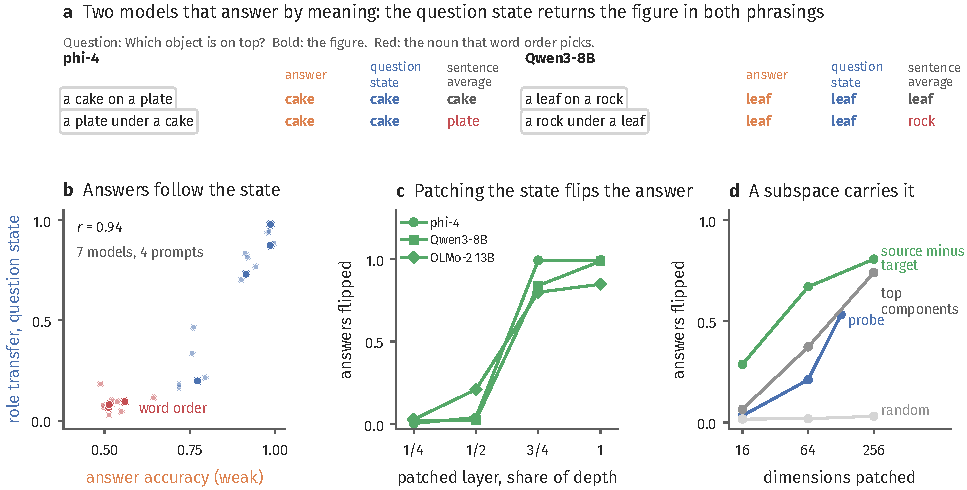
\includegraphics[width=0.76\textwidth]{fig_both.pdf}
  \caption{\textbf{Where a model answers by meaning, the answer runs through a recoverable question state.} \textbf{a.} Answers (orange) and figure probes of the question state (blue) and of the token average (grey) for two pairs of new nouns; bold marks the figure and red the ground. \textbf{b.} Answer accuracy against role transfer of the question state, for seven models on the main prompt (large dots) and three others (small dots). \textbf{c.} Patching the question state from a source with the opposite figure flips the answer from the later layers on. \textbf{d.} At each model's selected layer, the top directions of the source--target difference flip more answers than the figure probe or the top principal components, and random directions almost none. Means over 3 seeds (2 in \textbf{d}).}
  \label{fig:both}
\end{figure*}

Asked which object is on top in ``a cake on a plate'' and in ``a plate under a cake'', phi-4 answers \emph{cake} both times, and a probe of its question state returns \emph{cake} both times (Figure~\ref{fig:both}a). Over new nouns and five relations, phi-4 and Qwen3-8B answer with accuracy 0.99, OLMo-2 13B with 0.92 and OLMo-2 7B with 0.77. The question states of the first three transfer the role at 0.98, 0.87 and 0.73, and across four prompts and seven models, transfer tracks accuracy at $r = 0.94$ (Figure~\ref{fig:both}b). With invented words such as \emph{blicket}, phi-4 still answers at 1.00 and transfers at 0.75. Appendix Figure~\ref{fig:case_lm} follows four sentence pairs through five models.

\textbf{The question builds the shared role code.} At the period that ends the sentence, before any question, a figure probe transfers at only 0.12--0.23 in these four models, although it returns the figure of canonical sentences at 0.96--1.00. At the question, the asked role transfers at 0.81--0.98 in phi-4 and Qwen3-8B. The unasked role transfers at 0.56--0.61 in phi-4, 0.44--0.50 in Qwen3-8B and 0.12--0.32 in OLMo-2, where a score below 0.5 means the probe returns the asked noun. The answer runs through this state. Patching it from a source with the opposite figure flips the answer on 0.99, 0.84 and 0.80 of pairs at three quarters of the depth, and on at most 0.21 in the first half of the layers. (Figure~\ref{fig:both}c,d).

\textbf{Models that answer by word order fail in both places.} Every Pythia and GPT-2 model, from 160 million to 12 billion parameters, answers at 0.41--0.56, and their question states transfer at 0.07--0.10. In every language model, a figure probe of the average over tokens transfers at 0.00--0.05, against 0.15 at initialization, and kernel and MLP probes do no better. Sentence states therefore carry the figure through codes that change with the phrasing. OLMo-2 7B marks the limit of a linear probe. It answers by meaning on 0.77 of pairs, and patches carry its answer, yet ridge, kernel and MLP probes transfer at most 0.51. H1 fails for these probes, and Observation~\ref{prop:subset} holds only for a probe that contains the model's later layers.

\subsection{Harnesses Repair Behavior Where Their Code Assigns the Roles}
\label{sec:harness}

A harness wraps a model in code that splits a task into calls \citep{zhang2025rlm,zhang2026harness}, so a system's decomposer can sit in code. When the model copies each sentence into first object, relation and second object, and code assigns the roles from a lexicon of the training relation phrases, Pythia-1.4B rises from 0.51 to 0.98 and OLMo-2 7B from 0.77 to 1.00, while held-out phrases such as ``atop'' fall back to the model's answer. When a planner names the figure and GLIGEN draws each noun in its box \citep{li2023gligen,lian2024llmgrounded}, the figure lands in its place on 0.92--0.93 of images in both phrasings with the lexicon, phi-4 or Qwen3-8B as planner, against 0.52 for SD 1.5, and on 0.50--0.51 with Pythia, GPT-2 or the first-mentioned noun.

\textbf{A harness moves the decomposer and leaves our test in force.} The plan holds each held-out noun as an explicit copy in its role, yet the lexicon is a lookup over relation words, weak by Lemma~\ref{lem:lookup}, and a harness that leaves the roles to the network, such as one yes-or-no question per noun, inherits its binding (Appendix~\ref{app:harness}). Our test therefore applies to whichever component assigns the roles, code included.

%=====================================================================
\section{A Shared Language for Compositionality}
\label{sec:spectrum}

\begin{figure*}[t]
  \centering
  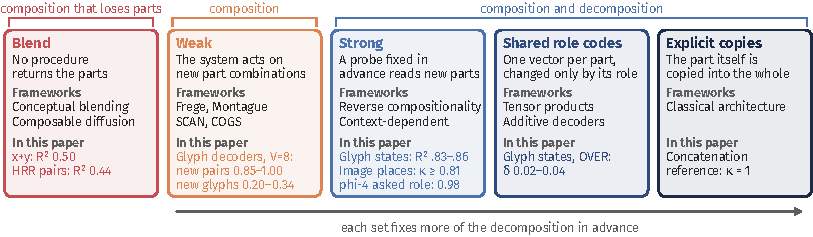
\includegraphics[width=0.66\textwidth]{fig_spectrum.pdf}
  \caption{\textbf{Accounts of compositionality differ in the capabilities they ask for.} Each card names a set of capabilities, its demand on decomposition, the accounts that ask for it and the systems of this paper that meet it.}
  \label{fig:spectrum}
\end{figure*}

\textbf{Five sets of capabilities.}\label{sec:sets} A \emph{blend} keeps no decomposition in roles. \emph{Weak compositionality} asks the system to act correctly on new combinations of training parts. \emph{Strong compositionality} further asks a linear probe, fixed in advance, to return every part in every role for parts new to it. \emph{Shared role codes} further require each part to enter every whole through one vector that changes only with its role, which lets a written vector or an edit act on one role alone. \emph{Explicit copies} further require that vector to be the part itself \citep{fodor1988}. The states of each set support every capability of the sets before it, although a system exhibits those capabilities only when its own procedures use its states.
Five conditions, checked in order, place any account, and Appendix Table~\ref{tab:spectrum} places twenty-two (Appendix~\ref{app:sets}). An account whose decomposer sees only training parts is weak, because a lookup passes.

\textbf{Modern tests score the weak form.} Generalization benchmarks such as SCAN and COGS test new combinations of training primitives, even in their new-role splits, because a known part in a new role is a new combination \citep{lake2018,kim2020cogs}. Winoground and ARO score matching through a pooled embedding \citep{thrush2022winoground,yuksekgonul2023}, text-to-image evaluation scores the end of a chain from text encoder to detector \citep{huang2023t2i,ghosh2023geneval}, and composable diffusion sums its concepts symmetrically, so swapping them leaves every generated latent identical \citep{liu2022composable}. Mechanistic tests reach the strong form once they fix their map in advance and score it on parts new to it \citep{geiger2021,mccoy2019}. Appendix Table~\ref{tab:modern} names the strong version of each test.

\begin{table}[t]
  \caption{\textbf{Each system placed under roles by position and by meaning.} Image and denoiser entries under meaning use moved photographs. $^\ast$phi-4 and Qwen3-8B. $^\dagger$For held-out nouns; the lexicon is a lookup over relation words. Sentence $\kappa$: Appendix~\ref{app:origins}.}
  \label{tab:tested}
  \centering\footnotesize
  \begin{tabularx}{\columnwidth}{@{}P{0.30\columnwidth}YY@{}}
    \toprule
    System & Roles by position & Roles by meaning \\
    \midrule
    Sentence states & Partial ($\kappa \le 0.58$) & Short of strong \\
    Question states$^\ast$ & Strong & Strong, asked role \\
    Image quadrants & Strong, fixed places & Low (0.18--0.49) \\
    Denoisers & Strong, fixed places & Low ($\le 0.21$) \\
    SD, PixArt images & Short of weak & Short of weak \\
    Lumina images & Partial (0.69--0.74) & Partial (0.54--0.69) \\
    Lexicon harness & Explicit copies$^\dagger$ & Explicit copies$^\dagger$ \\
    \bottomrule
  \end{tabularx}
\end{table}

\textbf{Modern systems bind roles to position.} In every pretrained state we tested, the parts sit in slots set by position: the order of mention in sentences and the absolute location in images. These states pass a probe test on new parts under a positional role assignment, yet they fail the converse paraphrase and lose most of their recoverability in a moved scene, two tests that Definition~\ref{def:decomp} requires because roles follow meaning. A role code by meaning appears only at the question, mostly for the asked role. Each system therefore receives a pair of placements (Table~\ref{tab:tested}), as binding IDs in language models \citep{feng2024} would.

%=====================================================================
\section{A Benchmark for Strong Compositionality}
\label{sec:benchmark}

A benchmark for the strong form changes the parts it holds out, the scores it reads and the way it assigns roles, in five components.

\begin{enumerate}[leftmargin=*,itemsep=1pt,topsep=0pt,partopsep=0pt]
  \item \textbf{Held-out parts.} Split the parts before fitting anything, and keep test parts out of every fitted procedure, the probe included. Held-out combinations of training parts cannot detect decomposition, because a lookup passes them (Lemma~\ref{lem:lookup}).
  \item \textbf{Two scores per whole.} Score the system's own output and a probe of its state, with the kind of probe fixed in advance and the state reported as $\kappa$ beside the same model with random weights. The pair locates a failure in the state or in the procedure that reads it (Section~\ref{sec:states}).
  \item \textbf{Roles that move.} Pair every whole with a converse paraphrase or a moved scene that keeps its meaning, and declare the role assignment. Without such pairs, positional binding passes (Sections~\ref{sec:images} and~\ref{sec:behavior}).
  \item \textbf{Capabilities that need the parts back.} Place held-out parts in every role, add parts without replay, nest beyond the training depth and edit one role at a time. A lookup over training parts can do none of these (Appendix Table~\ref{tab:capabilities}).
  \item \textbf{A stated claim.} Report the set reached under each role assignment, with the probe, the part vectors and the held-out parts, and report $\delta$ for a claim of shared role codes.
\end{enumerate}

Our relation sentences give one instance, which pairs ``a tulip on a barrel'' with ``a barrel under a tulip'' over held-out nouns and scores both the answer and the question state. On it, OLMo-2 7B answers by meaning through a code that our linear probes miss, a case that a benchmark reading outputs alone cannot tell apart from phi-4. A harness enters such a benchmark as one more system, scored at the component that assigns the roles.

%=====================================================================
\section{Conclusion and Limitations}
\label{sec:discussion}

States kept parts that behavior lost, models that answered by meaning built the asked role at the question, every pretrained state we tested bound roles to position, and test-time harnesses repaired behavior as far as the component that assigned the roles.

Our results also suggest what a strongly compositional network needs: a state with room for every part (Propositions~\ref{prop:ceiling} and~\ref{prop:ey}), a reader trained on many distinct parts (Proposition~\ref{prop:span}), one code per part that every role shares and the system uses (Proposition~\ref{prop:systematic}; Section~\ref{sec:states}), a relation that stays invertible on its own outputs for nesting (Proposition~\ref{prop:depth}), and role codes that follow meaning.

\textbf{Limitations.} Our evidence covers only the systems we tested, and additions, new roles, nesting and code swaps rest on small trained networks alone. In pretrained models, parts are new only to the probe, apart from invented words, image encoders lack a tested repair, and attribute binding remains untested (Appendix~\ref{app:limits}).

%=====================================================================
\section*{Impact Statement}

This paper presents work whose goal is to advance the field of Machine Learning. Tests that separate weak from strong compositionality may help practitioners judge when a model will handle new parts and roles, and a positive score on our test does not certify that a deployed system behaves compositionally. There are many potential societal consequences of our work, none of which we feel must be specifically highlighted here.

\section*{AI Use Statement}

% AUTHOR: check this statement against your own record of AI use before submission.
We used a large language model assistant (Claude, Anthropic) throughout this project: to write and run experiment code, to aggregate and plot results, to search and summarize related work, and to draft and revise the manuscript. The author designed the framework and the experiments, directed every analysis, checked the reported numbers against the logged results and takes full responsibility for the content.

\bibliography{references}
\bibliographystyle{icml2027}

%=====================================================================
\newpage
\appendix
\onecolumn

\section{Case Studies}
\label{app:cases}
% Case studies: every example comes from saved outputs, chosen by the fixed rule stated in each caption.
Each figure in this appendix shows individual wholes behind the rates of Section~\ref{sec:results}. Every example comes from saved outputs and follows a fixed selection rule, stated in its caption, so the galleries show typical cases. They are too small to estimate rates, which the main text reports over hundreds of wholes.

\subsection{Text-to-Image Generation}
\label{app:case_generation}

\begin{figure}[!htbp]
  \centering
  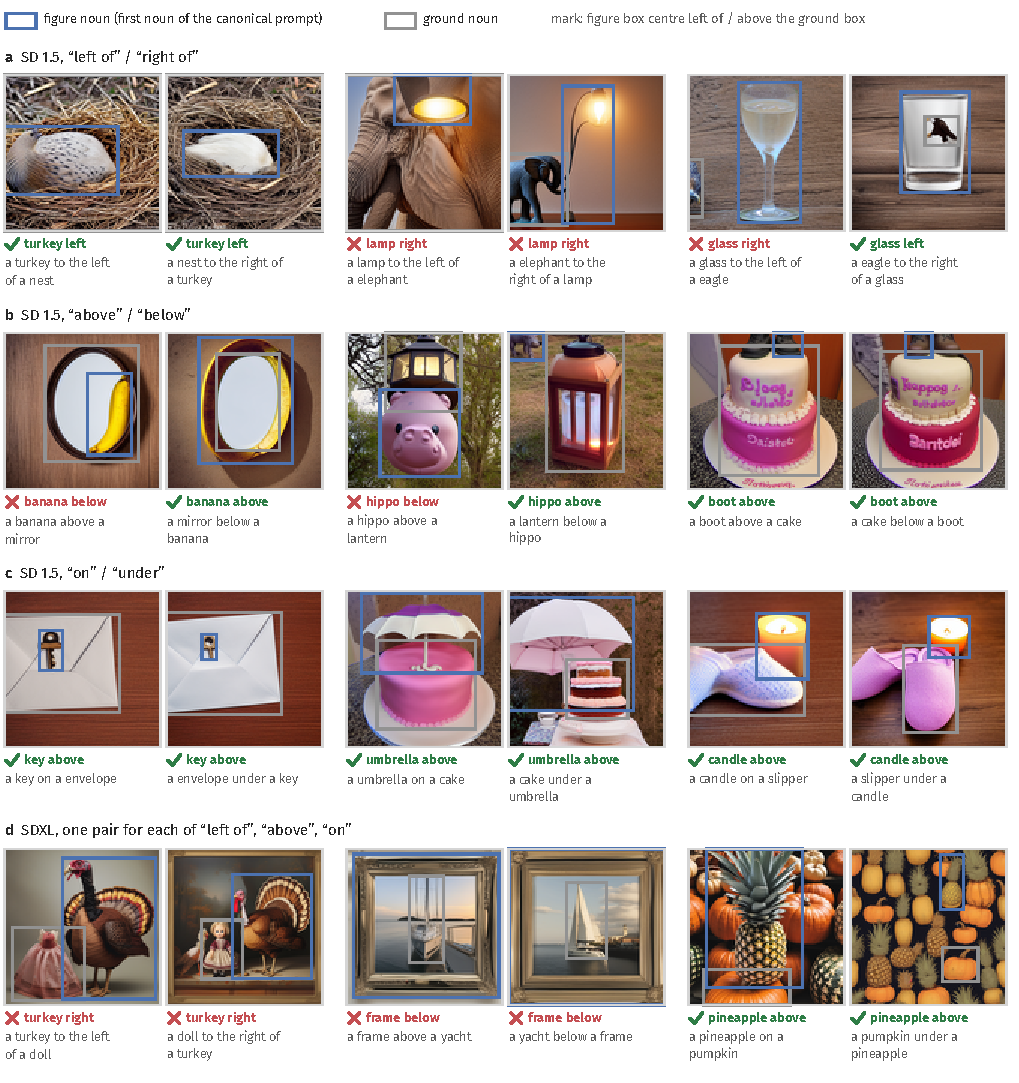
\includegraphics[width=\linewidth]{fig_case_generation.pdf}
  \caption{\textbf{Generated layouts ignore the relation word.} Each pair shows one prompt and its converse under the same seed (seed 0), with the detected boxes of the figure noun (blue) and the ground noun (grey), and a mark when the figure's box centre lies left of or above the ground's. The pairs are the first in index order, three per relation for SD 1.5 and one per relation for SDXL, whose two phrasings both hold both objects at the detection threshold of Section~\ref{sec:diffusion}. Prompts appear verbatim from the template, which writes ``a'' before every noun.}
  \label{fig:case_generation}
\end{figure}

Figure~\ref{fig:case_generation} shows the kinds of failure behind the rates of Section~\ref{sec:diffusion}. The lamp and the elephant keep one layout under both phrasings of \textsc{left of}, so the figure lands on the wrong side twice, while the turkey lands on the left of the nest under both phrasings. In three SD 1.5 pairs, the glass and the eagle, the banana and the mirror, and the hippo and the lantern, the figure lands in its place under one phrasing and out of it under the other, which a model that read the relation would avoid. Every \textsc{on} pair puts the figure on top in both phrasings, as stacking one object on the other would, and SDXL keeps the turkey and the frame on the wrong side in both phrasings and tiles the canvas with pumpkins in the converse of the last pair.

\begin{figure}[!htbp]
  \centering
  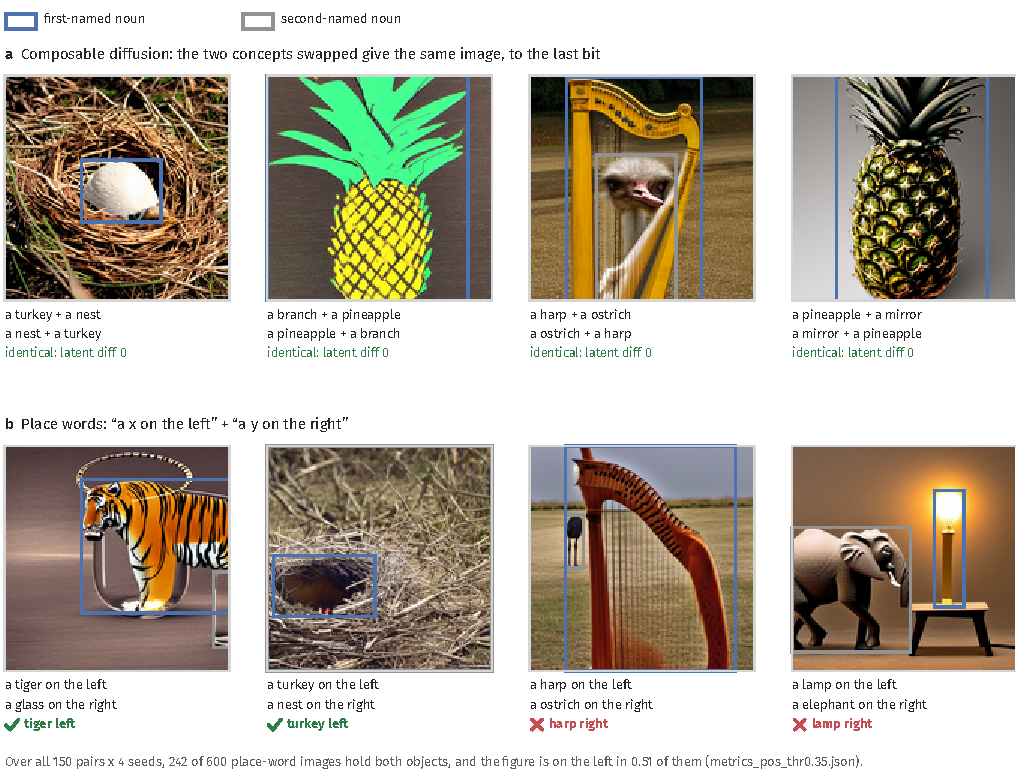
\includegraphics[width=\linewidth]{fig_case_compose.pdf}
  \caption{\textbf{Composable diffusion marks no roles, and place words do not fix one.} \textbf{a.} The first four pairs of the swap check: adding the two concepts' scores in either order gives the same latent to the last bit. \textbf{b.} Place words in each concept's prompt. The tiger pair comes from the main text, and the other three are the first pairs in index order with both objects detected at seed 0; the mark tells whether the figure sits on the left.}
  \label{fig:case_compose}
\end{figure}

Figure~\ref{fig:case_compose}a shows the symmetry of composable diffusion directly. Each swapped pair gives one image, because a sum of scores is the same in either order, so any role in the scene must come from the wording of each prompt. Place words supply such a wording, and Figure~\ref{fig:case_compose}b shows them succeeding for the tiger and the turkey and failing for the harp and the lamp. Over all 600 place-word images, 242 hold both objects, and the figure sits on the left in 0.51 of those.

\FloatBarrier
\subsection{Image Encoders}
\label{app:case_places}

\begin{figure}[!htbp]
  \centering
  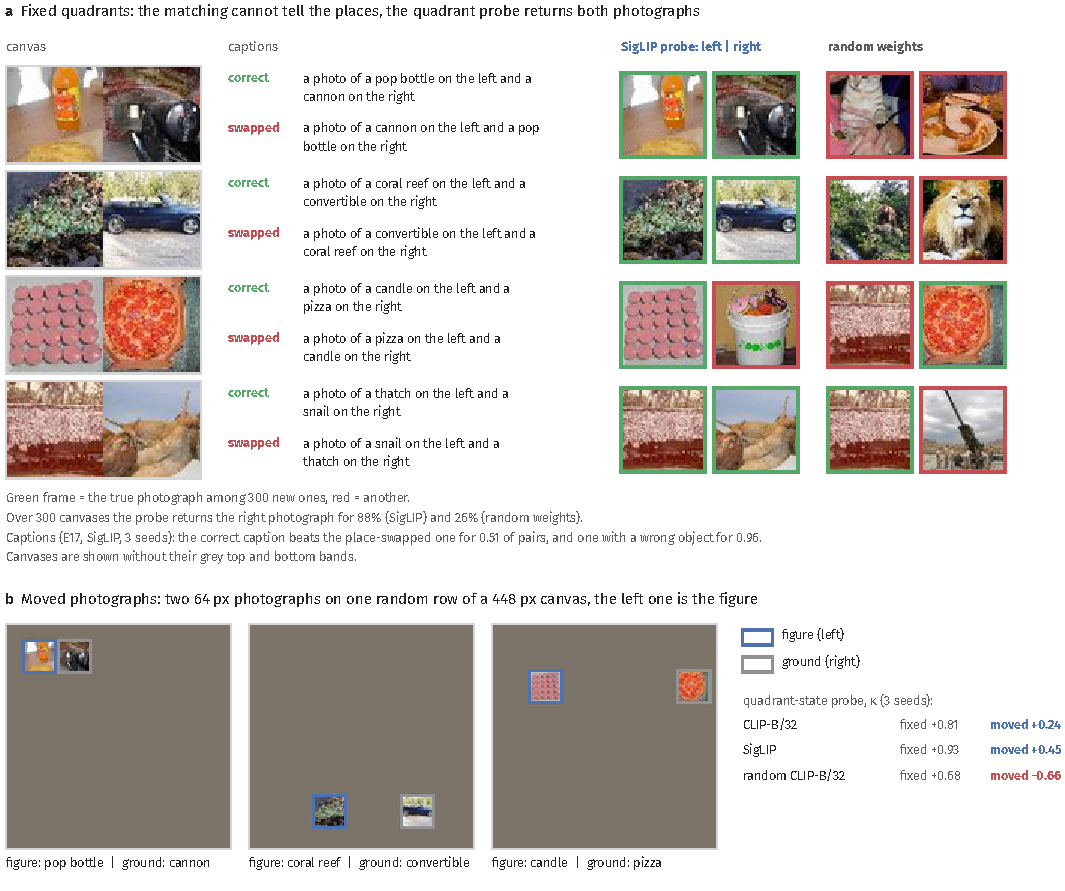
\includegraphics[width=\linewidth]{fig_case_places.pdf}
  \caption{\textbf{Image encoders keep fixed places that their matching ignores, and moving the photographs removes most of them.} \textbf{a.} The first four pairs of new photographs with named classes, each on a fixed-quadrant canvas, with the correct and the place-swapped caption, and the photographs that the linear probe of SigLIP's quadrant states returns for the left and the right role (green when correct among 300 new photographs), beside the same probe of a random-weight copy. \textbf{b.} The first three pairs placed as in the moved-photograph test of Section~\ref{sec:images}, where the left photograph is the figure, with $\kappa$ of the quadrant-average probe under fixed and moved placement (3 seeds).}
  \label{fig:case_places}
\end{figure}

In Figure~\ref{fig:case_places}a, SigLIP's caption matching prefers the correct caption over the place-swapped one on 0.51 of pairs, while its quadrant probe returns the right photograph in seven of the eight places shown and in 88\% of 300 canvases. The probe misses only the pizza, for which it returns a bucket. The random-weight copy returns the right photograph in two of the eight places and in 26\% of canvases. The moved canvases of Figure~\ref{fig:case_places}b show why the fixed quadrants overstate the role code. Two small photographs on one row can sit anywhere, so a place in the state no longer names a role, and $\kappa$ falls from 0.81 to 0.24 for CLIP-B/32 and from 0.93 to 0.45 for SigLIP.

\FloatBarrier
\subsection{Language Models}
\label{app:case_lm}

\begin{figure}[!htbp]
  \centering
  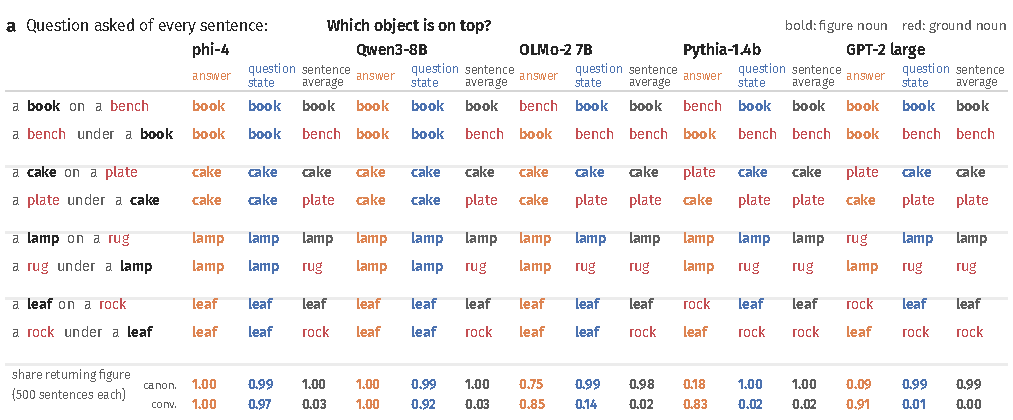
\includegraphics[width=\linewidth]{fig_case_lm.pdf}
  \caption{\textbf{Answers and states for four sentence pairs in five models.} The first four saved pairs of the relation \emph{on}/\emph{under}, each in its canonical and its converse phrasing, under the question ``Which object is on top?''. For each model, the answer (orange when it names the figure, red when it names the ground), the noun returned by the figure probe of the question state (blue when correct, red otherwise) and the noun returned by the same probe of the token-averaged sentence state (grey when correct, red otherwise). The bottom rows give the share returning the figure over 500 sentences of each phrasing.}
  \label{fig:case_lm}
\end{figure}

Figure~\ref{fig:case_lm} follows four sentence pairs through five models. phi-4 and Qwen3-8B name the figure in all eight sentences, and the figure probe of their question state returns the figure in all eight as well. Pythia-1.4b and GPT-2 large name the second-mentioned noun in seven of eight sentences, \emph{plate} for ``a cake on a plate'' and \emph{cake} for ``a plate under a cake'', and the probe of their question state returns the first-mentioned noun in every sentence, so answer and state both follow word order, from opposite ends of the sentence. OLMo-2 7B answers by meaning in seven of eight sentences, while its question-state probe returns the ground in three of the four converse sentences, the gap that Section~\ref{sec:behavior} traces to a role code that our linear probes miss. In every model, the probe of the token-averaged sentence state returns the first-mentioned noun, which is the figure in canonical sentences and the ground in converse ones.

\FloatBarrier
\subsection{Glyph Networks}
\label{app:case_glyph}

\begin{figure}[!htbp]
  \centering
  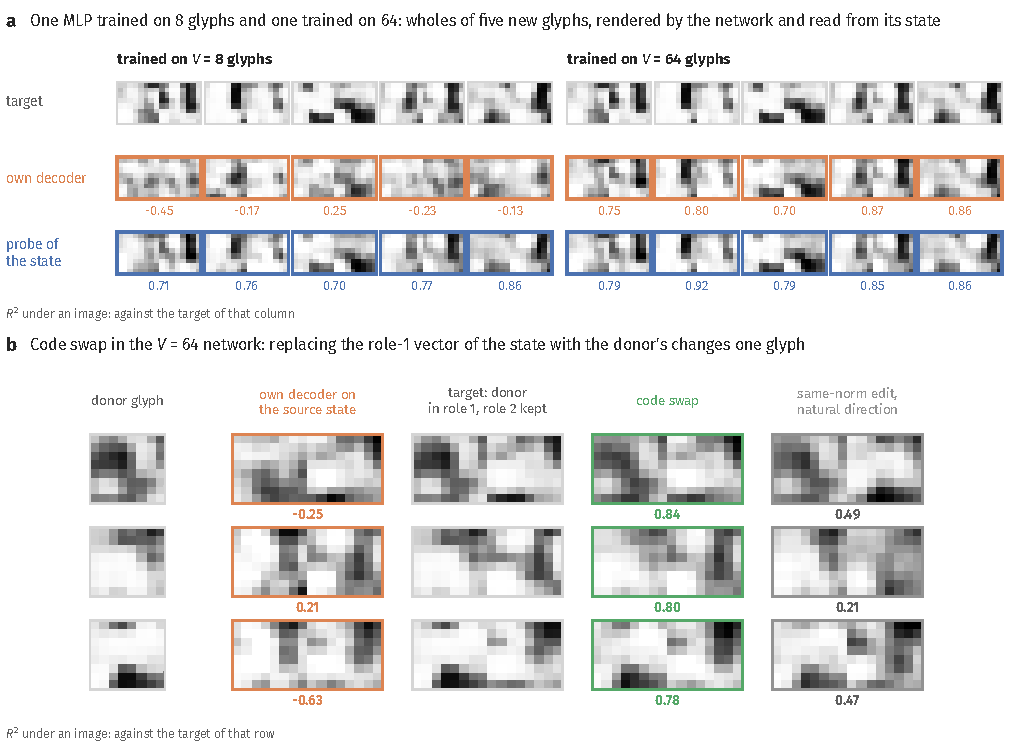
\includegraphics[width=\linewidth]{fig_case_glyph.pdf}
  \caption{\textbf{Glyph networks keep new glyphs their decoders cannot draw, and their decoders read the role codes.} \textbf{a.} Every saved whole of new glyphs for one MLP trained on 8 glyphs and one trained on 64 ($m = 64$, \textsc{over}, seed 0): the target, the network's own decoder and a linear probe of its state, with $R^2$ against each target. \textbf{b.} All three saved code swaps in the 64-glyph network: the donor glyph, the decoder on the source state, the target with the donor in role 1, the decoder after the code swap, and an edit of the same norm along the natural direction $h(a', b') - h(a, b)$, with $R^2$ against the target.}
  \label{fig:case_glyph}
\end{figure}

In Figure~\ref{fig:case_glyph}a, the decoder of the 8-glyph network misses most of each new glyph, with $R^2$ between $-0.45$ and 0.25, while a linear probe of the same state reconstructs each whole at 0.70--0.86. With 64 training glyphs the decoder catches up, at 0.70--0.87, and the probe stays at 0.79--0.92. In Figure~\ref{fig:case_glyph}b, writing a donor's vector into role 1 makes the decoder draw the donor in role 1 and keep the role-2 glyph, at 0.78--0.84 against the target, while an edit of the same norm along the natural direction reaches 0.21--0.49.
\FloatBarrier


\clearpage
\section{Related Work in Full}
\label{app:related}

\begin{figure}[t]
  \centering
  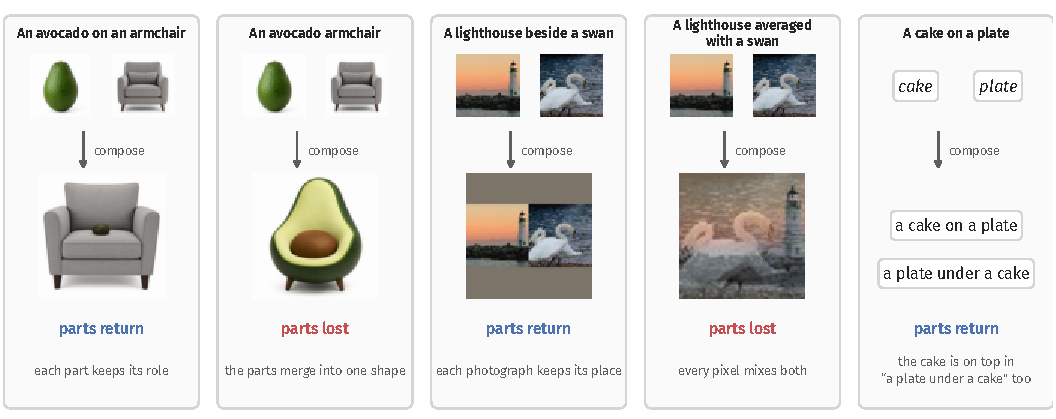
\includegraphics[width=\linewidth]{fig_intro.pdf}
  \caption{\textbf{Some wholes give their parts back, and others blend them.} Each column composes two parts into a whole. Placing an avocado on an armchair, setting two photographs side by side and naming two nouns in a sentence keep each part in its role, so the whole comes apart again (blue). An avocado-shaped armchair and the pixel average of two photographs merge the parts, and many pairs of parts give the same whole (red). Canva's text-to-image tool generated the avocado and armchair images \citep[after][]{openai2021dalle}, and the photographs come from Tiny-ImageNet \citep{le2015tiny}.}
  \label{fig:intro}
\end{figure}


\textbf{Compositionality of meaning.} Frege's principle holds that the meaning of a complex follows from the meanings of its parts and the way they combine \citep{frege1923}. \citet{montague1970} made the principle a homomorphism, a structure-preserving map from syntax to semantics \citep[see][]{janssen1997}. As a constraint on functions alone, however, the principle is vacuous, because a recoding of the parts makes any assignment of meanings compositional \citep{zadrozny1994}. Conceptual combination strains it from the other side. A guppy is a typical pet fish, yet neither a typical pet nor a typical fish \citep{osherson1981}, and conceptual blending builds wholes with structure of their own \citep{fauconnier2002}.

\textbf{Behavioral tests of composition.} The debate over composition in networks began with connectionist models of language \citep{rumelhart1986,pinker1988,elman1990}. \citet{marcus1998} argued that networks fail to extend a relation beyond their training space. Benchmarks now score a model's outputs on new combinations of training parts \citep{lake2018,keysers2020}, \citet{hupkes2020} divide the property into five tests, and meta-learning brings networks to the human level \citep{lake2023}. Detectors judge the scenes that text-to-image models generate \citep{ramesh2021,huang2023t2i}, and synthetic studies of concept learning follow how diffusion models acquire combinations of attributes \citep{okawa2023} and the rules of a random hierarchy \citep{favero2025diffusion}. All of these tests score outputs and leave the states unscored.

\textbf{Constituent structure.} \citet{fodor1988} argued that the systematicity and productivity of thought require representations whose constituents appear in every whole that contains them. \citet{smolensky1990} answered with tensor-product representations, which bind fillers to roles. With linearly independent roles, a linear map returns every filler exactly, even though the state holds no explicit copy of it. \citet{fodor1990} replied that such implicit constituents cannot act in processing, and the dispute continues \citep{goodale2026}.

\textbf{Context-dependent constituents.} \citet{smolensky1988} also described a looser kind of constituent. Subtracting \emph{cup without coffee} from \emph{cup with coffee} leaves coffee in the context of a cup, and this constituent differs in the context of a can or a tree. Smolensky called the two kinds strong and weak compositional structure \citep{smolensky1987}. His distinction concerns the form a constituent takes, whereas ours concerns the capabilities a state supports. In the same way, \emph{red} contributes differently to \emph{red hair} and to \emph{red apple} \citep{kamp1995}.

\textbf{Procedures that build and decompose.} \citet{vangelder1990} called a representation functionally compositional when general procedures build and decompose it. Reduced descriptions compressed part--whole hierarchies into single patterns \citep{hinton1990}. Recursive auto-associative memories learned the procedures \citep{pollack1990}, whereas vector-symbolic architectures fixed them by design \citep{plate1995,gayler2006,kanerva2009}. Models of analogy bind fillers to roles explicitly \citep{hummel1997}, although binding remains a problem for perception as well as for networks \citep{treisman1980,greff2020}.

\textbf{Reading parts from representations.} Probes decode constituents from states \citep{belinkov2022}, while tensor-product decompositions \citep{mccoy2019} and interchange interventions \citep{geiger2021} supply part vectors. Superposition lets a state carry more features than dimensions \citep{elhage2022}. Disentanglement seeks codes that separate the factors of variation \citep{bengio2013,locatello2019}, and identifiability results guarantee generalization for additive decoders \citep{lachapelle2023,wiedemer2024}. Yet decodable factors need not yield a decoder that generalizes \citep{montero2021}. We keep parts new to the probe and compare the probe with the system's own outputs.

\textbf{Measures of compositional structure.} Compression measures ask whether a composition of part vectors reproduces a representation \citep{andreas2019}. \citet{elmoznino2024} define representational compositionality as the compressibility of a representation into a short semantics over discrete sentences. \citet{elmoznino2026} score the structure that a whole reveals beyond its parts, a score near zero when the parts' structures already account for the whole. Both measures run from parts to whole and score the data themselves. Our measure runs from whole to parts and scores a system's state through a probe fixed in advance on parts new to it.


\section{Formal Results}
\label{app:proofs}

Throughout, a relation acts on parts $x_1, \ldots, x_k$ with codes in $\R^d$ and produces a state in $\R^m$. Stacking the codes gives $x = (x_1, \ldots, x_k) \in \R^{kd}$.



\begin{lemma}[Unrestricted coordinates reduce separability to injectivity]
\label{lem:psi}
Call $g$ separable if $\psi(g(x_1, \ldots, x_k)) = \sum_i \varphi_i(x_i)$ for some $\psi$ injective on the image of $g$ and some maps $\varphi_i$. If $\psi$ is unrestricted, every injective $g$ is separable.
\end{lemma}

\begin{proof}
Let $\varphi_i(x_i)$ place $x_i$ in the $i$-th block of $\R^{kd}$ and zeros elsewhere, so that $\sum_i \varphi_i(x_i) = x$. On the image of $g$ define $\psi = g^{-1}$, which exists because $g$ is injective; then $\psi(g(x)) = x = \sum_i \varphi_i(x_i)$.
\end{proof}

\noindent

\begin{lemma}[Lookup decodes any relation that is injective on a vocabulary]
\label{lem:lookup}
Let $\Voc$ be finite and let $g$ be injective on $\Voc^k$. Then the probe that matches a state to the stored table $\{g(t) : t \in \Voc^k\}$ returns every part of every whole of vocabulary parts.
\end{lemma}

\begin{proof}
Each state in the table has exactly one preimage in $\Voc^k$.
\end{proof}

\noindent



\begin{observation}[Behavior entails recoverability, and the converse fails]
\label{prop:subset}
Let a system's own procedures $\pi_1, \ldots, \pi_k$ read the state $h = g_r(x_1, \ldots, x_k)$ and return part vectors with error at most $\varepsilon$ in Eq.~\eqref{eq:recover} for parts drawn from $\D$. Then $r$ is $\varepsilon$-recoverable under every kind of probe $\U$ that contains the $\pi_i$. Conversely, for every $\varepsilon$-recoverable relation there is a system with the same state whose own procedures have error 1.
\end{observation}

\begin{proof}
The first claim holds with $u_i = \pi_i$ in Definition~\ref{def:recoverable}. For the second, let each own procedure return the constant $\mathbb{E}\,e(x)$, which has normalized error 1 and reads nothing from the state.
\end{proof}

\noindent
The first claim concerns the state the procedure reads, which in a language model is the state at the end of the question. It says nothing about a fixed class that excludes the procedure, such as linear probes of a state that a nonlinear decoder reads, and Appendix Definition~\ref{def:informative} also asks the part vector to be informative.

\begin{proposition}[Non-identifiability of linear blends]
\label{prop:fiber}
Let $g(x) = Ax$ with $A = [A_1 \cdots A_k] \in \R^{m \times kd}$, which covers symmetric blending, weighted addition, superposition, and HRR or MAP binding with fixed roles. If $\mathrm{rank}\,A < kd$, which holds whenever $m < kd$, then for every whole $z$ in the image of $g$ the parts with $g(x) = z$ form a translate of $\ker A$, of dimension $kd - \mathrm{rank}\,A \geq 1$, and no probe recovers the parts of every whole.
\end{proposition}

\begin{proof}
If $Ax_0 = z$, the solutions of $Ax = z$ are $x_0 + \ker A$, of dimension $kd - \mathrm{rank}\,A$ by rank--nullity. Any nonzero $n \in \ker A$ has a nonzero block $n_i$, so $x_0$ and $x_0 + n$ share the whole but differ in their $i$-th part.
\end{proof}

\begin{remark}
No continuous map from $\R^{kd}$ to $\R^m$ with $m < kd$ is injective, so the conclusion extends to continuous nonlinear relations; discontinuous injections exist. A tensor product with linearly independent roles has $\mathrm{rank}\,A = kd$.
\end{remark}

\begin{proposition}[Ceiling on new-part recovery]
\label{prop:ceiling}
Let $x \sim \mathcal{N}(0, I_{kd})$ and $z = Ax$. The probe that minimizes the expected squared error of $x_i$ given $z$, among all measurable functions, is linear, and its $R^2$ for role $i$ is
\begin{equation}
  R^2_i = \frac{1}{d}\,\mathrm{tr}\big(A_i^{\top} (A A^{\top})^{+} A_i\big), \qquad \frac{1}{k}\sum_i R^2_i = \frac{\mathrm{rank}\,A}{kd}.
\end{equation}
\end{proposition}

\begin{proof}
$x$ and $z$ are jointly Gaussian with $\mathrm{Cov}(x, z) = A^{\top}$ and $\mathrm{Cov}(z) = AA^{\top}$, so $\mathbb{E}[x \mid z] = A^{\top}(AA^{\top})^{+}z$, which is linear and is the minimum-mean-square-error estimator over all functions. Its residual covariance is $I - P$ with $P = A^{\top}(AA^{\top})^{+}A$, the orthogonal projection onto the row space of $A$. The variance of $x_i$ explained is the trace of the $i$-th diagonal block of $P$, which is $\mathrm{tr}(A_i^{\top}(AA^{\top})^{+}A_i)$, out of a total of $d$. Summing over blocks gives $\mathrm{tr}\,P = \mathrm{rank}\,A$.
\end{proof}

\noindent
For $x + \alpha y$ the ceiling is $1/(1 + \alpha^2)$ for role~1 and $\alpha^2/(1 + \alpha^2)$ for role~2; for $x + y$ it is $1/2$ for each; for HRR or MAP binding of two parts in $d$ dimensions with fixed roles it averages $1/2$; and for a generic projection into $m < kd$ dimensions it is close to $m/(kd)$ for each role. Figure~\ref{fig:measure}b compares these values with fitted probes. For Gaussian part vectors with covariance $\Sigma$, the same argument gives $R^2_i = \mathrm{tr}(\Sigma_i A_i^{\top}(A\Sigma A^{\top})^{+}A_i\Sigma_i)/\mathrm{tr}\,\Sigma_i$, where $\Sigma_i$ is the covariance of role $i$ and the roles are independent.

\begin{proposition}[Ceiling for any relation under linear probes]
\label{prop:ey}
Let the stacked part vectors $x \in \R^{kd}$ have finite second moments and covariance $\Sigma$ with eigenvalues $\lambda_1 \ge \cdots \ge \lambda_{kd}$, and let $h = g(x) \in \R^m$ for any measurable $g$. For any linear probes $u_i(h) = W_i h + b_i$, one per role,
\begin{equation}
  \frac{\sum_i \mathbb{E}\,\lVert u_i(h) - x_i \rVert^2}{\mathrm{tr}\,\Sigma} \;\ge\; \frac{\sum_{j > m} \lambda_j}{\mathrm{tr}\,\Sigma},
\end{equation}
so the variance-weighted mean $R^2$ over roles is at most $\sum_{j \le m} \lambda_j / \mathrm{tr}\,\Sigma$, which equals $\min(1, m/(kd))$ for isotropic codes.
\end{proposition}

\begin{proof}
Stack the probes into $u(h) = Wh + b$ with $W = [W_1; \ldots; W_k] \in \R^{kd \times m}$. Its values lie in the translate $b + \mathrm{range}\,W$ of a linear subspace of dimension at most $m$. For every fixed translate $L$ of a linear subspace of dimension at most $m$ and every random vector $y \in L$, $\mathbb{E}\,\lVert x - y \rVert^2 \ge \mathbb{E}\,\lVert x - \Pi_L x \rVert^2$, where $\Pi_L$ is the orthogonal projection onto $L$, and the right side is minimized over $L$ by the span of the top $m$ principal directions of $x$ through its mean, with value $\sum_{j > m} \lambda_j$ \citep{eckart1936}.
\end{proof}

\noindent
The bound does not depend on $g$ at all: it limits any linear function with an offset of any $m$-dimensional vector. Unlike Proposition~\ref{prop:ceiling}, it therefore holds for nonlinear relations, such as trained encoders, and for non-Gaussian parts. Nonlinear probes, which can exploit a nonlinear relation's curvature, escape it. In Section~\ref{sec:states} we compute it from the principal components of the declared part vector.

\begin{proposition}[Fitted linear procedures are determined only on the span of the fitted wholes]
\label{prop:span}
Let $g(x) = c + Bx$ with $B = [B_1 \cdots B_k]$ of full column rank, and let a linear procedure $u(h) = Wh + b$ be fitted to return the stacked part vectors $x_t$ exactly on wholes $t = 1, \ldots, n$. Let $T = \mathrm{span}\{x_t - \bar{x}\}$. Then every such $u$ returns $x$ exactly on wholes with $x - \bar{x} \in T$, and two such procedures can disagree arbitrarily on any whole with a component outside $T$. Because $T \subseteq S_1 \oplus \cdots \oplus S_k$, where $S_i$ is the span of the centred role-$i$ codes of the fitted wholes, new parts are recovered by every exact fit only if each $S_i = \R^d$, which requires at least $d + 1$ distinct parts in every role. Conversely, if $B$ has orthonormal columns (as for concatenation) and the fitted pairs vary each role independently enough that $T = S_1 \oplus \cdots \oplus S_k$, the minimum-norm fit returns $\bar{x}_i + \Pi_{S_i}(x_i - \bar{x}_i)$ for each role, so that for isotropic codes with mean zero $R^2_i = \dim S_i/d - \mathbb{E}\,\lVert (I - \Pi_{S_i})\bar{x}_i \rVert^2/d$. For general $B$ the minimum-norm fit returns the projection of $x - \bar{x}$ onto $T$ in the metric $B^{\top}B$, which mixes roles.
\end{proposition}

\begin{proof}
Exact fit means $WBx_t + Wc + b = x_t$ for all $t$; subtracting the mean gives $WBv = v$ for $v \in T$, which fixes $u$ on $\bar{x} + T$. Any $W'$ with $W'BT = 0$ can be added, together with the intercept $b' = -W'(c + B\bar{x})$, without changing the fit, and because $B$ is injective, $W'$ can be chosen to be nonzero on $B v$ for any $v \notin T$. The span of $V$ centred points has dimension at most $V - 1$. For the converse, the minimum-norm $W$ vanishes on $(BT)^{\perp}$ and inverts $B$ on $BT$, so $u(h) - \bar{x}$ is the $B^{\top}B$-orthogonal projection of $x - \bar{x}$ onto $T$; when $B^{\top}B = I$ this is the Euclidean projection, whose $i$-th block is $\Pi_{S_i}$ when $T$ is the direct sum. The error in role $i$ is then $(I - \Pi_{S_i})(x_i - \bar{x}_i)$, whose expected squared norm for isotropic $x_i$ independent of $\bar{x}_i$ is $d - \dim S_i + \mathbb{E}\,\lVert (I - \Pi_{S_i})\bar{x}_i \rVert^2$.
\end{proof}

\noindent
For concatenation of $V \le d + 1$ isotropic parts in $\R^d$, $\dim S_i = V - 1$ and $\mathbb{E}\,\lVert(I - \Pi_{S_i})\bar{x}_i\rVert^2 = (d - V + 1)/V$, so the minimum-norm probe has $R^2 = (V-1)/d - (d - V + 1)/(Vd)$ on new parts; for $V > d + 1$, $S_i = \R^d$ and $R^2 = 1$. The proposition concerns linear procedures; a nonlinear decoder learned from wholes is likewise unconstrained outside the region its training wholes cover, and the mechanism is the same. It predicts that the number of distinct parts governs whether a learned procedure transfers to new parts more than the number of observed combinations does (Figure~\ref{fig:strong}b). It also explains why a population estimate of Definition~\ref{def:recoverable} needs a probe-training pool of many more than $d$ parts.



\noindent

\begin{proposition}[Unbinding with shared role codes]
\label{prop:systematic}
Let $g(x_1, \ldots, x_k) = c + \sum_i B_i e(x_i)$ with $B = [B_1 \cdots B_k]$ of full column rank, and let $B^{+} = [P_1; \ldots; P_k]$ be its pseudo-inverse in row blocks. Then (i) $P_i(h - c)$ returns each part vector, $e(x_i) = P_i(h - c)$; (ii) for any permutation $\pi$ of roles, the state of the permuted whole is $h_\pi = c + \sum_i B_{\pi(i)} P_i (h - c)$, a linear function of $h$ with an offset; (iii) the contribution of a part observed only in role $i$ to any role $j$ is $B_j P_i (h - c)$ computed from any single whole containing it; and (iv) replacing the part in role $i$ changes $h$ only within the range of $B_i$ and leaves every probe value $P_j(h - c)$, $j \ne i$, unchanged.
\end{proposition}

\begin{proof}
(i) $B^{+}B = I$, so $B^{+}(h - c)$ returns the stacked part vectors. (ii) The permuted whole has state $c + \sum_i B_{\pi(i)} e(x_i)$; substitute (i). (iii) The same substitution with $j$ in place of $\pi(i)$. (iv) Only the term $B_i e(x_i)$ depends on $x_i$, and $P_j B_i = 0$ for $j \neq i$.
\end{proof}

\noindent
The proposition restates the unbinding property of tensor-product representations \citep{smolensky1990} for any relation with shared role codes, and the residual $\delta$ plays the role of the reconstruction error of a tensor-product decomposition network \citep{mccoy2019}. The code swaps of Section~\ref{sec:states} test separately whether a system uses that information when it acts.

\begin{proposition}[Approximate unbinding]
\label{prop:approx}
Let $h = c + Bx + \eta$ with roles exchangeable, so that the parts are independent and identically distributed across roles, and let $\hat{e}_i$ be any probes of the part vectors with $\varepsilon$ as in Eq.~\eqref{eq:recover} and $\delta$ as in Eq.~\eqref{eq:factor}. The predicted permuted state $\hat{h}_\pi = c + \sum_i B_{\pi(i)}\hat{e}_i(h)$ satisfies
\begin{equation}
  \mathbb{E}\,\lVert \hat{h}_\pi - h_\pi \rVert^2 \;\le\; 2\lVert B \rVert^2\, k\,\varepsilon\, \mathbb{E}\,\lVert e - \mathbb{E}\,e \rVert^2 + 2\,\delta\, \mathbb{E}\,\lVert g - \mathbb{E}\,g \rVert^2 .
\end{equation}
\end{proposition}

\begin{proof}
$\hat{h}_\pi - h_\pi = B_\pi(\hat{e}(h) - x) - \eta_\pi$, where $B_\pi$ permutes the blocks of $B$ and $\eta_\pi$ is the residual of the permuted whole. A block permutation is an orthogonal right factor, so $\lVert B_\pi \rVert = \lVert B \rVert$; $\mathbb{E}\,\lVert \hat{e}(h) - x \rVert^2 \le k\,\varepsilon\,\mathbb{E}\,\lVert e - \mathbb{E}\,e\rVert^2$ by Eq.~\eqref{eq:recover}; and $\mathbb{E}\,\lVert \eta_\pi \rVert^2 = \mathbb{E}\,\lVert \eta \rVert^2$ because the parts are exchangeable. The bound follows from $\lVert a + b \rVert^2 \le 2\lVert a \rVert^2 + 2\lVert b \rVert^2$.
\end{proof}

\noindent
With $\hat{e} = B^{+}(h - c)$ the first term is replaced by $\lVert B_\pi B^{+} \rVert^2 \le \mathrm{cond}(B)^2$ times $\mathbb{E}\,\lVert \eta \rVert^2$, so the conditioning of $B$ also matters. Only here do the quantities of Definitions~\ref{def:recoverable} and~\ref{def:factor} jointly bound the error of a predicted state, and Section~\ref{sec:states} measures both quantities without evaluating the bound.

\begin{proposition}[Depth]
\label{prop:depth}
Let leaves in $\R^d$ be lifted to $\R^w$ by a linear map and composed by $g(x, y) = Ax + By$ with $A, B \in \R^{w \times w}$, possibly different at each level. The map from the $2^n$ leaves of a balanced whole of depth $n$ to its state has rank at most $\min(w, 2^n d)$, so its kernel has dimension at least $2^n d - w$ (at least $(2^n - 1)d$ when $w = d$), and for Gaussian leaves the average new-leaf $R^2$ of any probe is at most $\min(1, w/(2^n d))$. For any relation, linear or not, the same bound holds for linear probes by Proposition~\ref{prop:ey}.
\end{proposition}

\begin{proof}
The map is linear from $\R^{2^n d}$ to $\R^w$, so its rank is at most $\min(w, 2^n d)$, and rank--nullity gives the kernel. The bound on $R^2$ is Proposition~\ref{prop:ceiling} applied to the composite linear map; the last statement is Proposition~\ref{prop:ey} with $m = w$ and $kd = 2^n d$.
\end{proof}

\noindent

\noindent
\textbf{Crosstalk in recursive HRR.} The prediction $1 - (2^n - 1)d/w$ of Section~\ref{sec:states} follows from a short calculation. Leaves $x \in \R^d$ are lifted to $xP$ by $P \in \R^{d \times w}$ with i.i.d.\ $\mathcal{N}(0, 1/w)$ entries, and two subtrees $a, b$ at height $h$ are composed as $(a \circledast \rho^h_1 + b \circledast \rho^h_2)/\sqrt{2}$, with unitary role vectors, for which circular convolution is an orthogonal map that circular correlation inverts exactly. Unbinding one path from the root, by correlation with that path's role vectors and multiplication by $\sqrt{2}$ at each level, returns the target leaf's lift plus, for each of the other $2^n - 1$ leaves, its lift transformed by a product of convolutions with unitary vectors. Each of these crosstalk terms has the norm of the leaf's lift, and the role vectors randomize the phases of its spectrum. The spectrum of a lifted Gaussian leaf is close to flat, so each term is close to isotropic and uncorrelated with the target and with the other terms. The probe applies the pseudo-inverse of $P$, which for $w \gg d$ is close to an isometry composed with the orthogonal projection onto the $d$-dimensional row space of $P$, and that projection keeps on average a share $d/w$ of an isotropic vector's squared norm. With leaf variance $d$, the expected squared error is therefore $(2^n - 1)d \cdot d/w$, and $R^2 \approx 1 - (2^n - 1)d/w$. The calculation ignores the departure of $P$ from orthonormal rows, of relative order $\sqrt{d/w}$, and is least accurate at small $w$, where the observed values fall below it.

%=====================================================================


\section{Additional Definitions and Results}
\label{app:defs}
\label{app:extra}

\begin{defbox}{Informative part vectors and productivity}{informative}
A part vector $e$ is \emph{informative} at tolerance $\tau$ if a linear probe of $e$ recovers a description $z(x)$ of the parts that does not depend on the system, with $R^2 \ge 1 - \tau$ on new parts. A relation is \emph{productive to depth $n$} if Definition~\ref{def:repcomp} holds when the parts are themselves wholes of depth up to $n - 1$, with the state of each whole as its part vector.
\end{defbox}

The informative requirement closes the loophole of Section~\ref{sec:repcomp}. The blend $(Px, Py)$, with $P$ a projection of rank $r < d$, discards $d - r$ dimensions of each part, yet it is exactly recoverable with the part vector $e(x) = Px$. An informative part vector rules this case out, because $Px$ fails to recover a description of $x$ itself. We report informativeness wherever such a description exists apart from the system, which holds for the glyph latents.

\textbf{The three limits in full.} A linear relation $g(x_1, \ldots, x_k) = A x$ with $A = [A_1 \cdots A_k]$ gives each whole a translate of $\ker A$ of decompositions, of dimension $kd - \mathrm{rank}\,A$ (Proposition~\ref{prop:fiber}). For Gaussian parts, no procedure of any kind recovers role $i$ with $R^2$ above $\mathrm{tr}(A_i^{\top}(AA^{\top})^{+}A_i)/d$, which gives 0.8 for role~1 of $x + 0.5y$ and 0.5 for $x + y$ (Proposition~\ref{prop:ceiling}). For any relation and part distribution, a linear probe of an $m$-dimensional state explains at most the share of the parts' variance in the top $m$ principal components of the stacked part vectors (Proposition~\ref{prop:ey}). A nested linear blend of depth $n$ into a state of width $d$ loses at least $(2^n - 1)d$ dimensions of its leaves (Proposition~\ref{prop:depth}). Recursive tensor products avoid this loss by raising the tensor rank, so their states grow with depth \citep{smolensky1990}.

\textbf{Width and relation set ceilings.} At $m = 8$, glyph states reach 0.67--0.71 against the ceiling of 0.79 from Proposition~\ref{prop:ey}. The non-additive \textsc{occlude} relation lowers recovery to 0.75--0.83.

\textbf{Asking for recovery over many parts improves behavior.} We add a linear head that recovers both glyphs of wholes built from 64 other glyphs to networks trained on 8 glyphs (Table~\ref{tab:objective}). The head improves both the state and the network's own decoder, which never sees those glyphs. The probe rises by 0.04--0.07 on plain inputs, by 0.12--0.13 on entangled inputs and by about 0.3 in the transformer. Read through a fixed renderer, the head reaches 0.92 and 0.70, above the 0.89 and 0.62 of networks trained end to end on 64 glyphs. The same head fitted on the training glyphs leaves the probe unchanged, as Proposition~\ref{prop:span} predicts. The 64 extra glyphs also give the encoder more data, so this result leaves open whether the objective beats plain training on the same parts.

\begin{table}[h]
  \caption{\textbf{A recovery objective over many parts improves the state and the network's own decoder, whereas one over training parts leaves the state unchanged.} Values are $R^2$ on new glyphs at $V = 8$, averaged over MLP, CNN and role--filler networks with 5 seeds. The fixed renderer draws the glyphs that the linear head predicts.}
  \label{tab:objective}
  \centering\small
  \begin{tabular}{@{}lcccccc@{}}
    \toprule
    & \multicolumn{3}{c}{Plain inputs} & \multicolumn{3}{c}{Entangled inputs} \\
    Objective & Probe & Own decoder & Renderer & Probe & Own decoder & Renderer \\
    \midrule
    None & 0.85 & 0.29 & --- & 0.54 & 0.13 & --- \\
    Training glyphs & 0.84 & 0.36 & 0.52 & 0.54 & 0.17 & 0.22 \\
    64 other glyphs & 0.90 & 0.47 & 0.92 & 0.66 & 0.39 & 0.70 \\
    \bottomrule
  \end{tabular}
\end{table}

\textbf{A random hierarchy supplies none of it.} In the random hierarchy model \citep{cagnetta2024rhm}, random rule tables expand a root symbol through levels of latent symbols into a string of tokens. We score linear probes of the one-hot string against vectors of the latents that the grammar alone fixes (Appendix~\ref{app:protocol}). Across 144 settings of vocabulary, rules per symbol, arity, depth, level and part vector, the input recovers the latents of new symbols with $R^2$ between $-0.63$ and $-0.03$, even though it recovers those of training symbols with up to 0.90. On this grammar, any recoverability in a trained network's state must come from training.

%=====================================================================


\section{Setup in Full}
\label{app:setup}

\subsection{Capabilities}
The harder capabilities on the spectrum all start from a whole and need its parts back. Every later use of a part passes through decomposition (Table~\ref{tab:capabilities}).
The harder capabilities on the spectrum all start from a whole and need its parts back. Every later use of a part passes through decomposition (Table~\ref{tab:capabilities}).
\begin{itemize}
  \item \textbf{New parts.} A whole that comes apart exposes each part, including parts its system never combined.
  \item \textbf{New parts in every role.} A part learned in one role enters another, because the part and its role come apart.
  \item \textbf{Additions without forgetting.} A new part enters through its own vector, so old wholes stay intact.
  \item \textbf{Nesting.} A whole that decomposes can serve as a part, so wholes nest inside wholes.
  \item \textbf{Inspection.} A decomposition shows the share each part donates to the whole, and an edit of that share changes one part alone.
\end{itemize}
\begin{table}[t]
  \caption{\textbf{The strong form supports every weak capability and adds those that need decomposition.} Each row names a capability, the weakest set of the spectrum that supports it in our tests and the test of this paper that scores it on new parts. Five sets order the spectrum: a blend that keeps no decomposition, then weak, strong, shared role codes and explicit copies (Section~\ref{sec:sets}). Shared role codes give each part one vector per role (Section~\ref{sec:mechanics}), so a written vector or an edit acts on one role alone. No system we tested reaches explicit copies.}
  \label{tab:capabilities}
  \centering\small
  \begin{tabularx}{\linewidth}{@{}P{0.25\linewidth}P{0.14\linewidth}Y@{}}
    \toprule
    Capability & Set & Test in this paper \\
    \midrule
    New combinations of training parts & weak & Glyph decoders on new pairs of training glyphs; role questions about sentences of nouns from pretraining; caption matching and captions chosen by denoising error for new pairs of photographs \\
    New parts & strong & Decoders and probes on wholes of new glyphs; probes of image and language states on nouns and photographs new to the probe (by position: fixed places; order of mention); answers about invented words \\
    A new part in every role & shared role codes & Writing a new glyph's vector into a role it never filled \\
    Additions without forgetting & shared role codes & Adding 32 glyphs in sequence by written vectors, against fine-tuning \\
    Nesting & strong & Recursive decomposers and probes at depths beyond training \\
    Inspection and editing & shared role codes & Swapping one role's vector in the state; patches of the question state \\
    \bottomrule
  \end{tabularx}
\end{table}


\subsection{Calibration on Toy Operators}
\label{app:calibration}
Toy operators check the measure where the answer is known in advance. We combine two Gaussian parts in $\R^{16}$ by fourteen operators, from role--filler binding (concatenation and a tensor product) through fixed-width superposition (random projections into $0.5$ to $1.5$ times $kd = 32$ dimensions, HRR and multiply--add--permute (MAP) binding \citep{plate1995,gayler2006,kanerva2009}, and $x + 0.5y$) to symmetric blends ($x + y$ and $x \odot y$) and a random $\tanh$ layer. We fit ridge, least-squares and MLP probes of the role-1 part on wholes built from a vocabulary of $V$ parts, with 5 seeds for each $V$.

\begin{figure}[t]
  \centering
  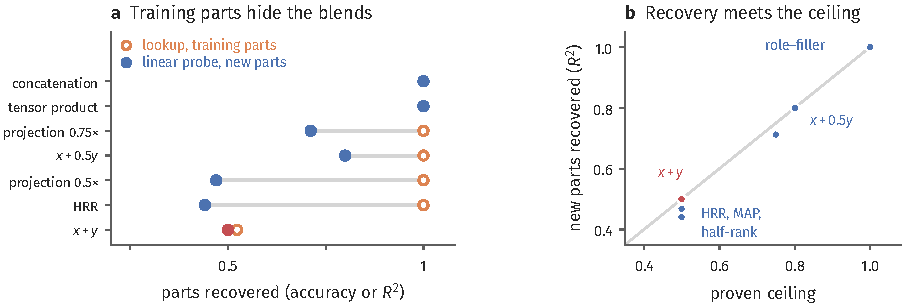
\includegraphics[width=\linewidth]{fig_measure.pdf}
  \caption{\textbf{Training parts hide blends, and new parts expose them.} \textbf{a.} A lookup over wholes built from 32 training parts (open orange) identifies the role-1 part of every operator except the symmetric blend, while a linear probe separates the operators on new parts (filled; red marks $x + y$). \textbf{b.} Linear recovery of new parts meets the ceiling of Proposition~\ref{prop:ceiling}. Means over 5 seeds.}
  \label{fig:measure}
\end{figure}

A lookup identifies the role-1 part of every operator that keeps the vocabulary distinct with accuracy 1.00, including half-rank projections and HRR, which keep only half of each part, and fails only on the symmetric blends, at 0.52 (Figure~\ref{fig:measure}a). A test on training parts therefore confuses role--filler binding with vector-symbolic superposition. At $V = 128$, linear probes recover the role--filler operators and full-rank projections at $R^2 = 1.00$, half-rank projections at 0.47 and $x + 0.5y$ at 0.80, its ceiling (Figure~\ref{fig:measure}b). HRR and MAP reach 0.44 and 0.47, close to their common ceiling of $1/2$. Flexible probes do worse because they memorize the vocabulary, and an MLP probe recovers only 0.11 of the half-rank projection on new parts, so every later test fixes a linear probe in advance.


\subsection{Systems, from toy to large}

We order the systems by how much control they give us (Table~\ref{tab:systems}). Toy networks trained from scratch let us keep parts new to the system itself and score its own outputs on them, so they test the hypotheses cleanly. Pretrained models saw their parts in pretraining, so parts are new only to the probe. For them we add random weights, training checkpoints and invented words as controls, and we ask whether the toy pattern recurs.

\begin{table}[t]
  \centering
  \small
  \caption{\textbf{Every system supplies parts, wholes and a state, and each supplies an output of its own.} Parts new to the system never entered its training, whereas parts new to the probe entered pretraining while staying out of the probe's fit. Invented words extend the language models' test to parts new to the model itself.}
  \label{tab:systems}
  \begin{tabular}{@{}p{0.14\linewidth}p{0.15\linewidth}p{0.16\linewidth}p{0.16\linewidth}p{0.16\linewidth}p{0.08\linewidth}@{}}
    \toprule
    System & Parts & Whole & State & Own output & New to \\
    \midrule
    Toy operators & Gaussian vectors in $\R^{16}$ & the operator's output on two parts & the output itself & lookup among training parts & probe \\
    Glyph networks & $8 \times 8$ glyphs & two glyphs on a canvas & encoder output $h \in \R^m$ & decoder's rendering & system \\
    Recursive composers & Gaussian leaves in $\R^8$ & binary tree of depth $n$ & root state & recursive decomposer & system \\
    Image encoders & Tiny-ImageNet photographs & two photographs on a canvas & patch states of each quadrant, or their average & matching captions through the pooled embedding, for image--text models & probe \\
    Diffusion models & the same photographs; nouns & a canvas; a caption naming two objects & denoiser features & generated images; choosing captions by denoising error & probe \\
    Language models & 305 concrete nouns & ``a $x$ on a $y$'' & question state; average over tokens & answering role questions & probe \\
    \bottomrule
  \end{tabular}
\end{table}

\paragraph{Glyph networks.} A fixed random generator renders a latent $z \in \R^{8}$ as an $8 \times 8$ glyph, and a whole places two glyphs on an $8 \times 16$ canvas under one of three relations. \textsc{beside} uses disjoint regions, \textsc{over} draws both glyphs in one region with the second mirrored, and \textsc{occlude} draws the second at half scale over the first. An encoder writes a state $h \in \R^m$, and a decoder renders the same parts in the same roles. The state serves as the system's representation, and the decoder as its own output. We train an MLP, a CNN, a transformer and a role--filler network, whose decoder renders each half of $h$ with one shared glyph decoder, at widths $m$ from 8 to 64 and vocabularies $V$ from 8 to 64 glyphs, with 9 seeds. With $V = 8$, two glyphs never fill role~2 in training, which removes 14 of the 56 ordered pairs of distinct glyphs, and a network trains on 34 of the remaining 42 until its training loss nears zero. The other eight pairs of the same glyphs test weak compositionality, and 256 wholes of glyphs outside its training test strong compositionality.

\paragraph{Recursive composers.} Balanced binary trees of depth $n$ carry Gaussian leaves in $\R^8$. A recursive auto-associative memory \citep{pollack1990} applies one learned composer at every node and one learned decomposer recursively, both trained on depths 1 and 2. The decomposer is the system's own output, and a probe maps the same root state to all $2^n$ leaves. For comparison, holographic reduced representations (HRR) of the same width $w$ use one pair of unitary role vectors per level, with 5 seeds for each $w$ from 16 to 256.

\paragraph{Pretrained models.} Sentences place two nouns in the roles of five asymmetric relations, such as ``a $x$ on a $y$'', and of the control ``a $x$ and a $y$''. We split 305 concrete nouns into 165 for training probes, 40 for validation and 100 new to the probe. Photographs come from Tiny-ImageNet \citep{le2015tiny}, whose 200 classes we split into 120, 30 and 50 in the same way. Two photographs share a $224 \times 224$ canvas, \textsc{beside} or \textsc{above} each other, or \textsc{overlap}ping. We test eleven text encoders from CLIP \citep{radford2021clip}, including those that condition Stable Diffusion \citep{rombach2022}, T5 \citep{raffel2020t5}, BERT \citep{devlin2019bert} and GPT-2 \citep{radford2019gpt2}. The image encoders are CLIP ViT-B/32 and ViT-H/14 \citep{radford2021clip,cherti2023}, DINOv2 small, large and giant \citep{oquab2024dinov2}, and SigLIP so400m \citep{zhai2023siglip}. The diffusion models are Stable Diffusion 1.5 and SDXL \citep{rombach2022}. The language models are Qwen3-8B \citep{yang2025qwen3}, OLMo-2 7B and 13B \citep{olmo2024olmo2}, phi-4 \citep{abdin2024phi4}, and seven Pythia models from 160 million to 12 billion parameters \citep{biderman2023pythia}, and the GPT-2 models also answer as language models. We also follow ten checkpoints of Pythia-1.4b, plus nine checkpoints each of Pythia-410m and of five PolyPythia reruns \citep{vanderwal2025polypythias}.

\paragraph{Roles by meaning.} Each relation has a \emph{converse} paraphrase that reverses the order of mention while keeping the meaning, such as ``a tulip on a barrel'' and ``a barrel under a tulip'' (Figure~\ref{fig:protocol}c). The tulip is the \emph{figure} in both sentences, and the barrel is the \emph{ground}. The language models answer questions such as ``Which object is on top?'' after four demonstrations with training nouns. A test prompt ends with ``Sentence: a tulip on a barrel. Question: Which object is on top? Answer: the'', and we call the model's state at that final token the \emph{question state}. Image--text encoders match a canvas against a caption that names its objects in their places and against the same caption with the places swapped. Text encoders match a sentence against its converse paraphrase and against the same paraphrase with the nouns exchanged.

\subsection{Protocol}

\begin{figure}[t]
  \centering
  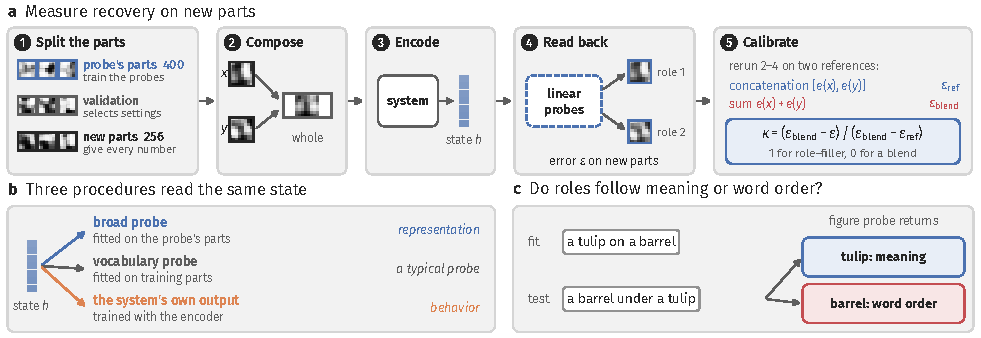
\includegraphics[width=\linewidth]{fig_protocol.pdf}
  \caption{\textbf{One protocol reads the same new parts through three procedures.} \textbf{a.} We split the parts before fitting anything (1). The system encodes wholes of two parts (2, 3), and linear probes fitted on the probe's training parts return each role's part from the state, with error $\varepsilon$ on new parts (4). The same steps, run on the concatenation and on the sum of the same part vectors, calibrate $\varepsilon$ into recoverability $\kappa$ (5). \textbf{b.} A probe trained on many parts measures the representation, a probe trained on the system's training parts stands in for a typical probe, and the system's own output measures behavior. \textbf{c.} A converse paraphrase keeps the figure and reverses the order of mention. A probe of the figure fitted on one phrasing therefore returns the tulip on the other if roles follow meaning, and the barrel if they follow word order. Colors keep one meaning in every figure. Orange marks the system's own output and blue a probe of its state. Green marks a procedure that reads through the state, such as a new decoder, an edit or a patch, grey marks controls and references, and red marks a blend or an answer by word order. Filled markers denote new parts and open markers training parts.}
  \label{fig:protocol}
\end{figure}

We split the parts before we fit anything. Probes and role maps fit wholes built from the probe's training parts, and new parts give every reported number. The probe class is linear and fixed before any result, and validation parts select only the ridge penalty, the layer and the part vector within that class. For a pretrained model, a part vector is the model's state for one part alone (``a $x$'', ``there is a $x$ here'', or the photograph), reduced to 16 principal components, each scaled to unit variance \citep{timkey2021}. For glyph networks, the part vector is the top 16 principal components of the glyph's pixels. Each system also runs with random weights, which keep its architecture, tokenizer and input format but remove learning. Every number is a mean over seeds, and Appendix~\ref{app:protocol} gives further details.

Two probes recur. The \emph{broad probe} trains on many parts, more than the dimension of the part vector, and measures the representation. The \emph{vocabulary probe} trains on the system's own training parts, as a typical probe would, and shows the ceiling that a procedure learned from that vocabulary faces (Proposition~\ref{prop:span}).

\subsection{Metrics}
\label{app:metrics}

Every metric scores wholes built from new parts.
\begin{itemize}
  \item \textbf{Recovery $R^2$.} For a procedure $u$ that returns a part vector, $R^2 = 1 - \varepsilon$ with $\varepsilon$ as in Eq.~\eqref{eq:recover}. The same score applies to probes, decoders and decomposers.
  \item \textbf{Recoverability $\kappa$.} Eq.~\eqref{eq:kappa} rescales a probe's error so that the sum of the part vectors scores 0 and their concatenation scores 1.
  \item \textbf{Role transfer.} A probe of the figure fits canonical sentences and reads converse ones. Role transfer is the share of converse sentences whose prediction $\hat{e}$ lies nearer the figure's vector than the ground's. Roles by meaning score 1, and word order scores 0.
  \item \textbf{Answer accuracy.} The share of questions on which the model prefers the correct noun by summed log-probability. Half of the questions ask for the figure and half for the ground, in both phrasings, so answering by word order scores 0.5.
  \item \textbf{Flip rate.} The share of pairs whose answer changes to the source's answer when we patch the question state, or one subspace of it, from a source prompt with the opposite figure.
  \item \textbf{Role residual $\delta$.} The share of a state's variance that the role maps of Eq.~\eqref{eq:factor} leave unexplained, so one shared code per role scores 0.
\end{itemize}


\section{Results in Full}
\label{app:results}
This appendix gives Section~\ref{sec:results} in full, with the controls that the main text summarizes.
We test the four hypotheses system by system, from the toy networks, where parts can be new to the system, to the pretrained models, where they are new only to the probe. Each system answers one question about the gap between behavior and state, and Table~\ref{tab:remedies} collects the repairs. Figure~\ref{fig:ladder} summarizes the first three hypotheses.


\subsection{Glyph networks keep new glyphs their decoders cannot draw}
\label{app:states}

Glyph networks come first because they are the one setting where a glyph can be new to the network itself. Only here can we tell whether a decoder that fails on a new glyph has lost the glyph or merely left it unread.

\textbf{Glyph networks act weakly.} Every architecture reproduces new pairs of training glyphs with output $R^2$ between 0.85 and 1.00, except the transformer trained on eight glyphs. New glyphs separate the networks by vocabulary. At $m = 64$, their output on new glyphs rises from 0.20--0.34 at $V = 8$ to 0.85--0.91 at $V = 64$ (Figure~\ref{fig:strong}b).

\textbf{Their states keep the new glyphs.} One MLP trained on 8 glyphs renders five wholes of new glyphs with a mean $R^2$ of $-0.15$, whereas a linear probe of its state recovers them with 0.76 (Figure~\ref{fig:strong}a shows four of them). Across the MLP, CNN and role--filler networks, the broad probe recovers 0.83--0.86 at $V = 8$ and 0.89 at $V = 64$, or $\kappa = 0.73$ and 0.83. The glyph's part vector carries the glyph, because a linear map of it recovers the latent with $R^2 = 0.92$. The transformer is the exception, at 0.59 for $V = 8$.

\textbf{The decoders behave like probes fitted on their vocabulary.} The vocabulary probe recovers only 0.23--0.29 of new glyphs at $V = 8$, and it tracks each network's own output better than the broad probe does. Proposition~\ref{prop:span} predicts this behavior, and it also predicts that distinct parts drive the decoder's reach. With 140 training pairs, moving from 16 to 64 glyphs raises the output on new glyphs from 0.47--0.64 to 0.81--0.82.

\textbf{A new decoder reads the state.} We freeze the encoder of each network trained on 8 glyphs and train a new decoder of the same architecture on wholes of 64 other glyphs. The new decoder renders new glyphs at 0.75, against 0.25 for the network's own decoder and 0.88 for networks trained end to end on 64 glyphs. Across architectures and vocabularies, the broad probe of a frozen encoder correlates with the output of its new decoder at $r = 0.87$, so recoverability predicts the procedures a state can support. Untrained encoders keep the glyphs almost as well and support an equally good new decoder (Section~\ref{sec:origins}), so in these small networks the gap sits in the decoder. Single glyphs teach the same lesson. Adding 64 other glyphs shown alone, each in one role with the other role blank, lets networks trained on all pairs of 8 glyphs render a new glyph alone with $R^2 = 0.88$, against $-0.30$ without them, and new pairs with 0.47, against 0.26.

\begin{figure}[t]
  \centering
  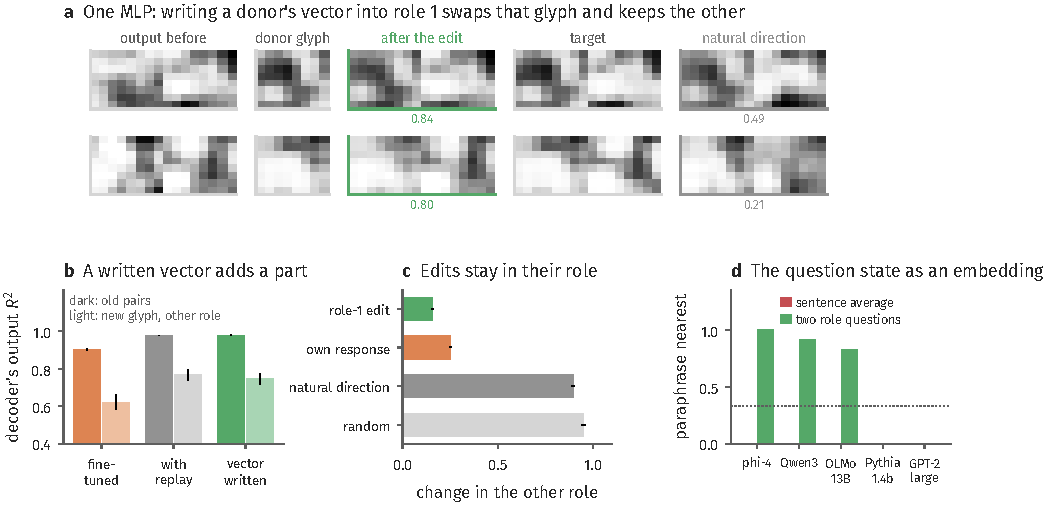
\includegraphics[width=\linewidth]{fig_decomp.pdf}
  \caption{\textbf{Procedures that read through role codes reuse the parts.} Role maps $h \approx c + B_1 e(x) + B_2 e(y)$, fitted on many glyphs, predict and edit states that each network's own decoder renders (\textsc{over}, $V = 64$). \textbf{a.} A code swap replaces the role-1 vector with a donor's vector, and the decoder renders the donor in role 1 while keeping the role-2 glyph. The natural direction $h(a', b') - h(a, b)$, scaled to the same norm, lands far from the target. Numbers give $R^2$ to the target. \textbf{b.} Writing a new glyph's vector through $B_2$ keeps old pairs (dark) and renders the new glyph in a role it never filled (light), with no gradient step, whereas fine-tuning damages both and replay needs stored data. \textbf{c.} A role-1 swap changes the role-2 half of the output less than other changes of the state do. \textbf{d.} In language models that answer by meaning, the state at two role questions places a sentence's converse paraphrase nearer than both role reversals, with no fitted probe, whereas the average over tokens never does; chance is $1/3$ (dotted). Means over 3--5 seeds, with standard errors.}
  \label{fig:decomp}
\end{figure}

\textbf{Swapping a role's vector changes one part.} Under \textsc{over}, the role residual $\delta$ is 0.02--0.04 for the MLP, CNN and role--filler networks and 0.06--0.13 for the transformer, so the states reach recoverability through shared role codes. A code swap writes a donor's vector into role 1, and the decoder renders the donor with $R^2 = 0.78$, against 0.81 when the network sees the donor itself (Figure~\ref{fig:decomp}a). The swap spills 0.16 into the untouched half of the output, against 0.90 for the natural direction $h(a', b') - h(a, b)$ (Figure~\ref{fig:decomp}c). The decoders therefore use the role codes, which answers the objection of \citet{fodor1990} for these systems. Under the non-additive \textsc{occlude}, $\delta$ rises to 0.11--0.22 and swaps spill 0.31.

\textbf{Written vectors add glyphs without forgetting.} We test additions twice. First, networks trained on 64 glyphs meet one new glyph in role~1 (Figure~\ref{fig:decomp}b). Fine-tuning on it damages the network, so the glyph in role~2 falls from 0.75 for the unmodified network to 0.62 and pairs of training glyphs fall from 0.98 to 0.90. Writing the glyph's vector into role~2 through $B_2$ takes no gradient step, so the old pairs stay at 0.98 while the decoder renders the glyph in a role it never filled at 0.75. Replay reaches 0.77, at the cost of stored data. Second, MLP, CNN and role--filler networks trained on 16 glyphs receive 32 new glyphs in sequence. Fine-tuning drops their old pairs to 0.18, as in catastrophic interference \citep{mccloskey1989}, whereas written vectors keep the old pairs at 0.99 and render each new glyph in a role it never filled at 0.71. Replay does better on the new glyphs, by 0.11--0.21, although it stores old data and takes gradient steps. A training objective that asks the state to give back many glyphs also helps the network's own decoder (Appendix~\ref{app:extra}).

\subsection{Recursive composers show the same gap at depth}
\label{app:depth}

Nesting is the capability that classical arguments for constituent structure lean on most \citep{fodor1988}, so we next ask whether the gap survives one level deeper than training.

\textbf{The decomposer fails beyond its training depths, and the root state does not.} Within its training depths, a recursive composer's own decomposer recovers new leaves almost perfectly for $w \ge 32$. At depth 3 it falls to $R^2 = 0.26$ at $w = 256$ after 6{,}000 steps, whereas a broad probe recovers the same leaves with 0.99 (Figure~\ref{fig:strong}c). At depths 4 and 5, which the composer never saw, the probe stays within 0.14 of the ceiling of Proposition~\ref{prop:depth}. HRR shows the same pattern by design. Recursive unbinding loses about $(2^n - 1)d/w$ of the variance to crosstalk and falls from 0.96 at depth 1 to $-0.13$ at depth 5, while a probe of the same state recovers the leaves exactly whenever $w \ge 2^n d$.

\textbf{Training at depth repairs the decomposer.} A decomposer that trains with its composer on trees of depth 3 to 5 recovers new leaves at 1.00, 1.00 and 0.97 at width 256, the values of the broad probe. Trained alone on the composer's states, the decomposer reaches only 0.74, 0.29 and 0.09, and no condition transfers to depth 6.

\subsection{Image encoders keep fixed places that their matching ignores}
\label{app:images}

The toy pattern would matter little if it vanished in models trained on the open world. Image--text encoders are a natural first test, because we score them by how well they match captions, a behavioral test of composition.

\textbf{Image encoders hold fixed places that their matching ignores.} CLIP-B/32, CLIP-H/14 and SigLIP prefer a caption that names the two new photographs over a caption with one wrong object, with accuracy 0.88--0.97. Against the caption with the two places swapped, however, they score 0.50--0.51, which is chance (Figure~\ref{fig:strong}d). Their quadrant states recover both photographs in their fixed places with $\kappa = 0.81$--$0.94$, and with 0.85--0.94 under \textsc{overlap}, against 0.29--0.72 for random weights across the encoders. The matching reads a single pooled embedding, and the average over patches, the closest state we probe, keeps far less of the places, at $\kappa = 0.17$--$0.49$ (Section~\ref{sec:origins}). Behavior agrees with the pooled state that the matching reads, and the recoverable state sits upstream, in the spatial map of the patch states. A matcher built on the quadrant states should close the gap for fixed layouts, and we leave that repair untested.

\textbf{Absolute positions carry most of these places.} A fixed quadrant ties each role to one location, so a probe can return the photographs by where they sit whether or not the state marks which one is the figure. To loosen this tie, we place both photographs at $64 \times 64$ pixels on one random row of a $448 \times 448$ canvas, at random horizontal positions, and the left photograph is the figure wherever the pair lands. With the same quadrant averages, part vectors and validation choices, the trained encoders recover both photographs in their roles with $\kappa = 0.24$ for CLIP-B/32, 0.42 for DINOv2-L and 0.45 for SigLIP, and a $4 \times 4$ grid of patch averages gives 0.18--0.49, against 0.81--0.93 for the same encoders under fixed quadrants. Random weights fall from 0.63--0.68 under fixed quadrants to $-0.17$ to $-0.71$, so their fixed-quadrant score came from location alone. The smaller photographs keep their identity, because features pooled within each photograph's box, taken in left-to-right order, still give 0.66--0.80. When the probe receives the two box features in random order and must find the figure itself, every encoder falls below zero, at $-0.08$ to $-0.17$. The trained encoders keep 0.18--0.49 of the relative places, and even this remainder may come from position, because a threshold on one photograph's horizontal position predicts the role with accuracy 0.84 and every encoder falls below zero when it must find the figure from the box features alone.

\subsection{Diffusion models keep fixed places that their own classifier ignores}
\label{app:diffusion}

Text-to-image diffusion models are the most cited case of machine composition after language models, and they supply an output of their own that reads the same canvases as the image encoders. A diffusion model scores a caption by how well it denoises an image under that caption, so the caption with the lower denoising error is the model's own choice \citep{li2023diffclassifier,clark2023diffclassifier}. We give Stable Diffusion 1.5 and SDXL the two-photograph canvases of Section~\ref{sec:images}, encoded by each model's autoencoder, and we compare captions over 25 timesteps from 50 to 950. The state is the denoiser's feature map from its middle and upsampling blocks, read with an empty caption and a fixed noise draw, and validation photographs choose the block and the timestep. SDXL runs at 512 pixels, below its native resolution.

\textbf{The model's own classifier ignores places.} Choosing by denoising error, SD 1.5 prefers the caption that names both photographs over a caption with one wrong object with accuracy 0.86--0.88, and SDXL with 0.69--0.71. Against the caption with the two places swapped, both models score 0.49--0.50, and no single timestep lifts either above 0.52. The denoising error sums over the whole map, and the next paragraph shows that the whole-map average of the features keeps little of the places.

\textbf{The denoiser's state keeps fixed places.} A linear probe of the denoiser's features, averaged within each quadrant, recovers both photographs in their fixed places with $\kappa = 0.70$ in SD 1.5 and 0.43 in SDXL (Figure~\ref{fig:ladder}). In SD 1.5 the score is 0.73 for \textsc{beside} and \textsc{above} and 0.66 for \textsc{overlap}. Averaged over the whole map, the same features give 0.13 and 0.05, so a reading that pools the whole map keeps almost none of the places. Behavior agrees with that low-recoverability reading, and the recoverable state sits upstream, in the spatial layout of the features. Under the relative places of Section~\ref{sec:images}, the places vanish from SD 1.5's state: quadrant averages give $\kappa = -0.06$ and the $4 \times 4$ grid gives $-0.14$. Box features in left-to-right order reach only 0.35, so the small photographs also lose much of their identity in the denoiser, and its places rest on fixed locations. SDXL remains untested under relative places.

\textbf{Training builds the places into the state.} Read against the trained model's part vectors, the same ones that the trained, random and latent comparison uses throughout, the autoencoder's latent, which is the denoiser's input, gives $\kappa = -0.48$ in SD 1.5 and $-0.47$ in SDXL, and the denoiser under random weights gives 0.12 and 0.09. Against the trained model's part vectors, training builds recoverability beyond the input and beyond random weights, as in the other pretrained models (Section~\ref{sec:origins}). As a stated caveat, a random denoiser read against its own part vectors reaches 0.80 and 0.83, because its vector for a single photograph keeps low-level detail that a linear probe matches easily.

\textbf{Generation ignores the relation as well.} We ask SD 1.5 for 150 pairs of new nouns in three relations, such as ``a cherry to the left of a tire'', in the canonical phrasing and in its converse, ``a tire to the right of a cherry'', with four seeds each, and we locate both objects with a detector \citep{liu2024groundingdino}. SD 1.5 often fuses the two objects or omits one, so about 200 images per relation and phrasing hold both objects as separate boxes. Among these, the figure lands in its place with accuracy 0.47--0.56 in every relation and phrasing, and the first-mentioned noun takes the first place equally often, at all three detector thresholds we tried. Under a shared seed, the two phrasings give the same layout for 0.63--0.75 of pairs, so the noise and the nouns set the layout and the relation word leaves it in place. SDXL at its native 1{,}024 pixels, with 50 pairs and two seeds per relation and phrasing, repeats the pattern for \textsc{above} and \textsc{left of}, at 0.46--0.55. For \textsc{on} it places the figure with accuracy 0.62--0.63 in both phrasings, from about 70 images each, which a habit of stacking one object on the other could explain, and it often tiles the canvas with copies of both objects, which makes a test by box centers crude. Read within each detected box of SD 1.5's own images, the denoiser's features name the noun only weakly, at $\kappa = 0.14$--$0.15$ against 0.71 for images of a single object, and figures and grounds score alike.

\textbf{The caption encoder accounts for part of this failure.} The denoiser reads the caption through CLIP-L, whose averaged caption state follows word order: a probe fitted to return the figure of canonical captions returns it for 0.95 of new noun pairs at the last layer and for 0.08 of their converses.

\textbf{Composable diffusion and place words fail in the same way.} Swapping the two concepts of a composable-diffusion sum leaves every generated latent identical to the last bit, which the arithmetic of the sum guarantees. A place added to each prompt, as in ``a tiger on the left'' and ``a glass on the right'', puts the figure in its place with accuracy 0.51. ``At the top'' and ``at the bottom'' give 0.53 on the noun pairs of \textsc{above} and 0.42 on those of \textsc{on}, and guidance weights from 3 to 12 leave the left/right accuracy at 0.36--0.48, although only 39--47 images per weight hold both objects.

\subsection{Language models build the asked role where they answer by meaning}
\label{app:behavior}

Language models let us test the first hypothesis where behavior succeeds. A model that answers role questions by meaning must, by H1, hold the role in the state it answers from.


\textbf{Models that answer by meaning carry the role in the question state.} Asked which object is on top in ``a cake on a plate'' and in ``a plate under a cake'', phi-4 answers \emph{cake} both times, and a probe of its question state also returns \emph{cake} both times (Figure~\ref{fig:both}a). Over new nouns and five relations, phi-4 and Qwen3-8B answer with accuracy 0.99, OLMo-2 13B with 0.92 and OLMo-2 7B with 0.77, in either word order. The question states of the first three transfer the role at 0.98, 0.87 and 0.73, in the same order as their accuracy. Across four prompts and seven models, role transfer correlates with answer accuracy at $r = 0.94$ (Figure~\ref{fig:both}b). Within a single model the correlation is 0.88, so a prompt that changes a model's answers also changes its transfer.

\textbf{The question builds the shared role code.} Before the question, the sentence holds the nouns in codes that change with the phrasing, and the next token names the figure, so the question itself could create a code shared by both phrasings. Two controls test this in phi-4, Qwen3-8B and both OLMo-2 models, with 3 seeds and the same rule for choosing the layer. At the period that ends the sentence, before any question, a figure probe transfers the role at only 0.12--0.23, and at most 0.36 at the best layer, although the same probe returns the figure of canonical sentences of new nouns with accuracy 0.96--1.00. Read from the question state, a probe for the role left unasked, the ground under the figure question or the figure under the ground question, transfers at 0.56--0.61 in phi-4, 0.44--0.50 in Qwen3-8B and 0.12--0.32 in the OLMo-2 models, where a score below 0.5 means that the probe returns the asked noun, which in the converse phrasing is also the noun in the ground's word position. The asked role transfers at 0.81--0.98 in phi-4 and Qwen3-8B, and only phi-4 carries part of the unasked role.

\textbf{Patching the question state moves the answer.} We replace the final-token state with the state from a source prompt whose figure is the other noun. At three quarters of the depth, the answer flips on 0.99 of pairs in phi-4, 0.84 in Qwen3-8B and 0.80 in OLMo-2 13B, and at the last layer on 0.99, 0.99 and 0.85 (Figure~\ref{fig:both}c). A source with the same figure leaves the answer in place on 0.78--1.00 of pairs. Patches in the first half of the layers flip at most 0.21, so the answer reaches this token late. Patching the probe's 16 dimensions changes the noun that the probe returns, yet it flips at most 0.06 of answers, and the probe's 64 and 128 dimensions flip 0.21 and 0.53 on average (Figure~\ref{fig:both}d). The top 64 directions of the difference between source and target, fitted on other nouns, flip 0.76, 0.75 and 0.51 of answers, against at most 0.03 for 64 random directions.

\textbf{Answers reach parts new to the model.} With invented words such as \emph{blicket} in place of the nouns, phi-4 answers with accuracy 1.00, Qwen3-8B with 0.98, OLMo-2 13B with 0.79 and OLMo-2 7B with 0.71. Role transfer falls to 0.75, 0.66, 0.53 and 0.41 in the same order. An invented word takes about 2.5 tokens, against 1.1 for a real noun, so the question state must gather each invented word from several tokens, which may explain the lower transfer.

\begin{figure}[t]
  \centering
  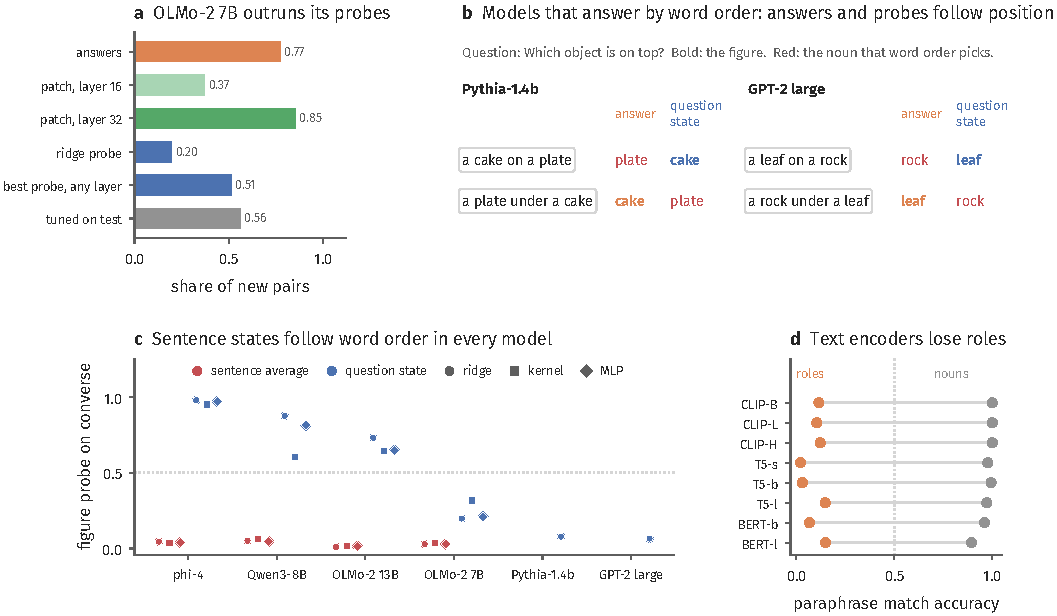
\includegraphics[width=\linewidth]{fig_weak.pdf}
  \caption{\textbf{Behavior can outrun a linear probe, and sentence states fail both tests.} \textbf{a.} OLMo-2 7B answers by meaning (orange), and its question state carries the answer under patching (green), while ridge, kernel and MLP probes of that state miss the role (blue), even with hyperparameters chosen on the test set (grey). \textbf{b.} Pythia-1.4b and GPT-2 large answer with the last-mentioned noun, and probes of their question states return the first-mentioned noun. Bold marks the figure and red the ground. \textbf{c.} A figure probe of the average over tokens returns the noun in the figure's word position (red) in every language model and for every probe, while the same probe at the question returns the figure (blue). \textbf{d.} Text encoders tell a sentence's nouns from others (grey), yet they prefer a sentence's converse paraphrase over the same paraphrase with the nouns exchanged on only 0.02--0.15 of pairs (orange), where matching meaning scores 1. New nouns; means over 3 seeds.}
  \label{fig:weak}
\end{figure}

\textbf{Models that answer by word order fail in both places.} Pythia-1.4b answers \emph{plate} for ``a cake on a plate'' and \emph{cake} for ``a plate under a cake'', the last-mentioned noun each time (Figure~\ref{fig:weak}b). A probe of its question state returns the first-mentioned noun each time. Every Pythia and GPT-2 model answers role questions at 0.41--0.56, from 160 million to 12 billion parameters and at every checkpoint of Pythia-1.4b. Their question states transfer the role at 0.07--0.10.

\textbf{Sentence states follow word order in every model.} A figure probe of the average over tokens transfers at 0.00--0.05 in every language model, against 0.15 at initialization, so training strengthens the binding to word order (Figure~\ref{fig:weak}c). Kernel and MLP probes do no better, at 0.00--0.06. The trained states carry the figure, but through codes that change with the phrasing, so these states lack shared role codes for meaning. Text encoders fail the same way. They tell a sentence's nouns from other nouns with accuracy 0.89--1.00, yet they prefer the converse paraphrase over the noun-swapped paraphrase on only 0.02--0.15 of pairs (Figure~\ref{fig:weak}d).

\textbf{OLMo-2 7B marks the limit of a linear probe.} OLMo-2 7B answers by meaning on 0.77 of pairs, while a ridge probe of its question state transfers the role at only 0.20 (Figure~\ref{fig:weak}a). Patches show that the state carries the answer. They flip 0.37 of answers at layer 16, where we fit the probe, and 0.85 at layer 32. Ridge, kernel and MLP probes at layers 16 to 32 transfer at most 0.51, and 0.56 with hyperparameters chosen on the test set. The answer thus depends on a role code that none of our probes reads, so H1 fails for these probes in OLMo-2 7B. Observation~\ref{prop:subset} still holds for a probe that contains the model's own later layers. Recoverability therefore depends on the kind of probe we fix.

\textbf{The question state serves as an embedding.} We read the question state at the end of two questions, one asking for the figure and one for the ground, and use the pair as a sentence embedding. With no fitted probe, this embedding places the converse paraphrase nearer than both role reversals for 100\% of pairs of new nouns in phi-4, 92\% in Qwen3-8B and 83\% in OLMo-2 13B (Figure~\ref{fig:decomp}d). The same embedding fails in Pythia-1.4b and GPT-2 large, whose answers follow word order.

\begin{table}[t]
  \caption{\textbf{Reading through the state repairs the failing procedures of glyph networks and recursive composers, and gives language models a sentence embedding that carries the role.} Values are $R^2$ of the system's output for the glyph and recursive networks, and the share of pairs of new nouns whose converse paraphrase is nearer than both role reversals for the language models. Each row compares runs within one experiment. Glyph values average MLP, CNN and role--filler networks over 5--9 seeds, and the sequence of 32 glyphs starts from networks trained on 16 glyphs. Recursive values use width 256, 5 seeds and 20{,}000 training steps, which give 0.27 at depth 3 against 0.26 after 6{,}000 steps in the text, and language-model values use 3 seeds.}
  \label{tab:remedies}
  \centering\small
  \begin{tabularx}{\linewidth}{@{}P{0.25\linewidth}P{0.24\linewidth}YY@{}}
    \toprule
    Repair & Failure it targets & Without & With \\
    \midrule
    Train a new decoder on a frozen state & Decoder fails on new glyphs & 0.25 & 0.75 \\
    Learn parts from single parts & Decoder fails on new glyphs & New glyph alone $-0.30$, new pair 0.26 & 0.88 and 0.47 \\
    Add parts by writing vectors & Fine-tuning forgets old pairs & Old pairs 0.18 after 32 glyphs & Old pairs 0.99; new glyph in a new role 0.71 \\
    Train the decomposer with its composer at each depth & Decomposer fails one level deeper & $0.27$, $-0.08$, $-0.29$ at depths 3--5 & 1.00, 1.00, 0.97 \\
    Read the role from two question states & The token-averaged sentence state follows word order & Paraphrase nearest for no pair & 1.00 phi-4, 0.92 Qwen3-8B, 0.83 OLMo-2 13B \\
    \bottomrule
  \end{tabularx}
\end{table}

\subsection{Where recoverability comes from}
\label{app:origins}

A state can hold its parts because the input already held them, because the architecture keeps them apart, or because training put them there. We compare each state with its input and with the same architecture under random weights (Figure~\ref{fig:origins}). For the glyph networks we add \emph{entangled inputs}, which pass each whole through a fixed random map before the encoder, three rounds of an orthogonal rotation and $\tanh$ at gain 4.

\begin{figure}[t]
  \centering
  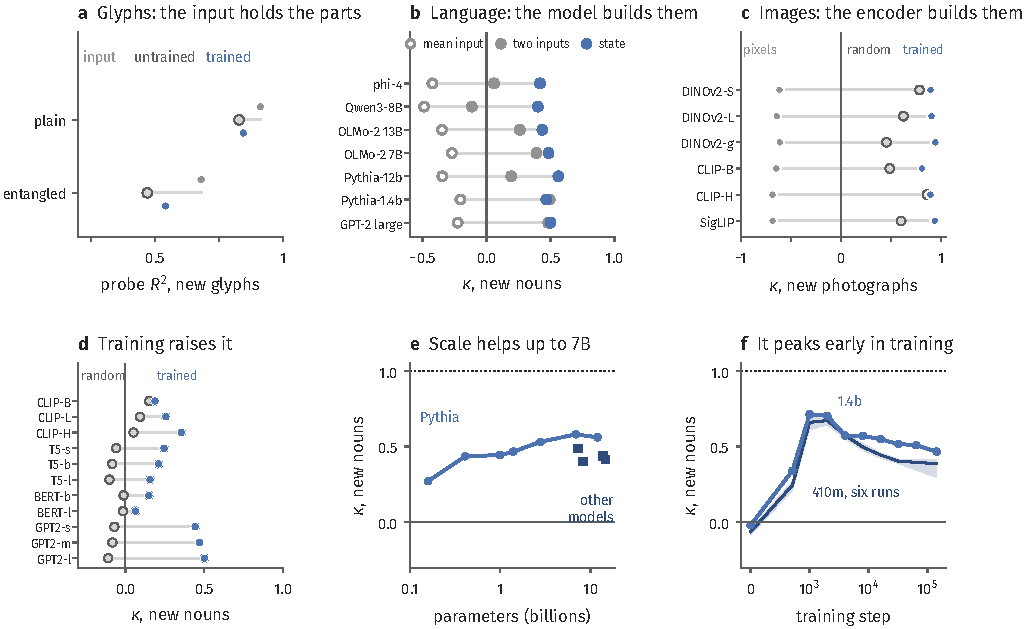
\includegraphics[width=\linewidth]{fig_origins.pdf}
  \caption{\textbf{The input supplies recoverability in the glyph networks, whereas pretrained models build it beyond their inputs.} Each row compares a trained state (blue) with its input (grey) and with random weights (light grey). \textbf{a.} Probes of new glyphs at $V = 8$, on plain inputs and on inputs entangled by a fixed random map. \textbf{b.} Language models against the average and the concatenation of the two nouns' input embeddings. \textbf{c.} Image encoders against raw pixels, scored with each encoder's own part vectors. \textbf{d.} Text encoders. \textbf{e.} Pythia models of growing size, whose scale trend is Pythia's alone, and four other language models (squares). \textbf{f.} Training of Pythia-1.4b, where step 0 is the initialization, and of Pythia-410m from six random seeds (line and range). Probes in \textbf{b} and \textbf{d}--\textbf{f} recover the nouns in their order of mention. $\kappa$ is 1 for the concatenation of the part vectors (dotted) and 0 for their sum. Means over 3--5 seeds.}
  \label{fig:origins}
\end{figure}

\textbf{Glyph networks inherit recoverability from their input.} The input pixels reach $R^2 = 0.91$ and untrained networks 0.82--0.83, and a frozen untrained encoder even supports an equally good new decoder, at 0.75 (Figure~\ref{fig:origins}a). Training in these small networks therefore mostly shapes the decoder. A fixed random map that entangles the input lowers the input's own probe to 0.68. The MLP, CNN and role--filler networks then reach $R^2 = 0.54$--$0.55$, which is 0.06--0.08 above untrained encoders and 0.13--0.15 below the input. No condition we tried lifts a state above its input. Recovery predicts the output of a new decoder, with $r = 0.98$ on entangled inputs.

\textbf{Pretrained models build recoverability beyond their input.} Averaging a sentence's input embeddings gives $\kappa = -0.21$ to $-0.49$ for the nouns in their order of mention across seven language models (phi-4, Qwen3-8B, OLMo-2 13B and 7B, Pythia-12b, Pythia-1.4b and GPT-2 large), below the sum of the part vectors. Concatenating the two nouns' input embeddings, which grants each noun's location, gives $-0.12$ to 0.49. States averaged over tokens exceed this baseline in five of the seven models and match it in GPT-2 large and Pythia-1.4b (Figure~\ref{fig:origins}b). For photographs, raw pixels give $\kappa = -0.61$ to $-0.69$ against the encoder's part vectors, which no linear map reaches from pixels, far below the quadrant states at 0.81--0.94 and below random weights at 0.29--0.72 across the encoders (Figure~\ref{fig:origins}c). Because raw pixels cannot reach semantic part vectors by construction, the comparison with random weights carries the claim for images.

\textbf{Training builds recoverability of the nouns in their positions, and Pythia's scale trend runs up to about 7 billion parameters.} Among the text encoders, the GPT-2 models reach $\kappa = 0.44$--$0.50$, CLIP-H 0.36 and the others 0.06--0.26, against $-0.11$ to $0.15$ under random weights (Figure~\ref{fig:origins}d). Within Pythia, $\kappa$ rises from 0.27 at 160 million parameters to 0.56--0.58 at 6.9 and 12 billion and levels off between those two sizes, while Qwen3-8B, OLMo-2 and phi-4 reach 0.40--0.49 and show no scale trend of their own (Figure~\ref{fig:origins}e). Pythia-1.4b peaks at 0.71 after 1{,}000 steps, 0.7\% of training, and then declines to 0.47. Six runs of Pythia-410m peak at about the same point (Figure~\ref{fig:origins}f). These probes recover the nouns in the order of mention, as the next paragraph shows, so these values score positional binding and leave the role by meaning to Section~\ref{sec:behavior}.

\textbf{Word order and architecture supply part of it.} Causal attention keeps the tokens of the first noun from seeing the second, so random weights in GPT-2 and CLIP already recover the first-mentioned noun alone with $\kappa = 0.50$--$0.58$, while the second falls to $-0.26$ to $-0.75$ and the average over roles stays at $-0.11$ to $0.15$. The control ``a $x$ and a $y$'' gives the same $\kappa$ as the asymmetric relations in every encoder, so these probes recover the nouns in their order of mention, which is a positional binding. In image encoders the choice of state decides recovery. Trained encoders reach $\kappa = 0.17$--$0.49$ in their states averaged over patches and 0.81--0.94 in their quadrant states, because the patch states keep two photographs apart whereas the average over patches blends them.


\section{The Spectrum in Full}
\label{app:spectrum}
\begin{table}[tp]
  \caption{\textbf{Each account asks for the set of capabilities that its demand on decomposition sets} (sets of Figure~\ref{fig:spectrum}).}
  \label{tab:spectrum}
  \centering\footnotesize
  \begin{tabularx}{\linewidth}{@{}P{0.34\linewidth}YP{0.22\linewidth}@{}}
    \toprule
    Account & Demand on decomposition & Set \\
    \midrule
    Conceptual blending and combination \citep{fauconnier2002,osherson1981,kamp1995} & Parts need not return intact & Blend \\
    Composable diffusion \citep{liu2022composable} & Symmetric sum of concept scores & Weak in parts, blend in roles \\
    \addlinespace
    Frege, Montague \citep{frege1923,montague1970} & Fixes the build, asks nothing of the way back & Weak \\
    Generalization benchmarks \citep{lake2018,kim2020cogs,keysers2020,hupkes2020,lake2023} & Outputs on new combinations & Weak \\
    Vision--language benchmarks \citep{thrush2022winoground,yuksekgonul2023} & Matching against swapped roles & Weak \\
    Text-to-image evaluation \citep{ramesh2021,huang2023t2i,ghosh2023geneval} & Generated outputs against the prompt & Weak \\
    Concept-space studies \citep{okawa2023,park2024hidden,favero2025diffusion} & Learning of new combinations in synthetic data & Weak \\
    Compositional reasoning tests \citep{dziri2023,press2023} & Answers that chain known facts & Weak \\
    Recursive auto-associative memories \citep{pollack1990} & Learned decomposer at trained depths & Weak; root state can be strong \\
    Vector-symbolic architectures \citep{plate1995,gayler2006,kanerva2009} & Unbinding and clean-up against a vocabulary & Weak; strong while width holds every part \\
    \addlinespace
    Reverse compositionality \citep{fodor2002} & Understanding a whole requires its parts & Strong \\
    Functional compositionality \citep{vangelder1990} & General procedures build and decompose & Strong \\
    Context-dependent constituents \citep{smolensky1988} & Parts return through codes that change with context & Strong without shared codes \\
    Decodable factors \citep{montero2021} & A probe recovers what the decoder fails to combine & Strong state, weak decoder \\
    Mechanistic tests \citep{lepori2023,geiger2021,geiger2024das,mccoy2019} & Maps from states to parts & Strong once the map is fixed and scored on new parts \\
    Sparse dictionary features \citep{cunningham2023sparse,bricken2023monosemanticity,park2024linear} & Features add linearly and carry no roles & Strong in parts, blend in roles \\
    Object-centric slots \citep{locatello2020slot} & Exchangeable slots lose roles & Strong in parts, blend in roles \\
    \addlinespace
    Tensor-product representations \citep{smolensky1990} & Independent role vectors, linear unbinding & Shared role codes \\
    Disentanglement, additive decoders \citep{bengio2013,lachapelle2023,wiedemer2024} & One coordinate block or sum term per factor & Shared role codes \\
    Compression and Kolmogorov measures \citep{andreas2019,elmoznino2024,elmoznino2026} & Composed parts reproduce the whole on training data & Shared role codes, tested by composing \\
    Binding IDs \citep{feng2024} & A shared code per entity set by position & Shared role codes by position \\
    \addlinespace
    Classical constituent structure \citep{fodor1988} & Constituents appear in every whole & Explicit copies \\
    \addlinespace
    Probes \citep{belinkov2022,hewitt2019}, recodings \citep{zadrozny1994} & No fixed probe, or no new parts & Outside; every injective system passes \\
    \bottomrule
  \end{tabularx}
\end{table}

We place twenty-two accounts on one spectrum, ordered by the capabilities each asks for (Figure~\ref{fig:spectrum}, Table~\ref{tab:spectrum}).

\subsection{Five sets of capabilities}
\label{app:sets}

A \emph{blend} keeps no decomposition in roles. \emph{Weak compositionality} acts correctly on new combinations of training parts. \emph{Strong compositionality} further asks a linear probe, fixed in advance, to return every part in every role for parts new to it (Definition~\ref{def:decomp}). \emph{Shared role codes} further give each part one vector that changes only with its role (Definition~\ref{def:factor}), and \emph{explicit copies} make that vector the part itself \citep{fodor1988}. In our tests, explicit copies add a form without adding a capability, because the concatenation reference already reaches $\kappa = 1$.

\textbf{Placing a new account.} Five conditions, checked in order, place any account. (a) An account that scores no decomposition of the whole sits in the weak set when it scores outputs on new combinations and in the blend set when it composes parts without marking roles. (b) An account whose decomposer sees only training parts is weak, because a lookup passes. (c) An account with no probe class fixed in advance lies outside the spectrum, and one with a fixed class is strong. (d) An account whose role codes share one vector per part, with $\delta \approx 0$, asks for shared role codes. (e) An account whose whole tokens each constituent explicitly asks for explicit copies. Split verdicts such as ``weak in parts, blend in roles'' arise when an account meets different conditions for parts and for roles. Of the five tests of \citet{hupkes2020}, systematicity falls in the weak set, productivity maps to nesting in the strong set, substitutivity maps to the converse-paraphrase test, and localism and overgeneralisation are behavioral tests outside the spectrum.

\subsection{Modern tests and methods}
\label{app:modern}

\begin{table}[t]
  \caption{\textbf{Behavioral test families score the weak form, and mechanistic tests can reach the strong form.} Each row gives what the family scores, what it cannot see and the change that would test the strong form.}
  \label{tab:modern}
  \centering\small
  \begin{tabularx}{\linewidth}{@{}P{0.21\linewidth}YYY@{}}
    \toprule
    Family & Scores & Cannot see & Strong version \\
    \midrule
    Generalization benchmarks (SCAN, COGS, CFQ, SLOG) & Outputs on new combinations & Whether the state keeps each primitive & Probe each role on new primitives \\
    Vision--language benchmarks (Winoground, ARO) & Matching against swapped roles & Places inside the encoder & Probe the patch states \\
    Text-to-image evaluation (T2I-CompBench, GenEval) & Detected objects, attributes, places & The stage of the chain that loses a part & Probe the denoiser's state \\
    Composable diffusion (a composition method) & Presence of each concept & Roles, which a symmetric sum never marks & Tie each concept to a role \\
    Reasoning tests (compositionality gap) & Answers chaining two facts & Whether the intermediate state holds both & Probe and patch it \\
    Mechanistic tests (subnetworks, interventions) & Maps from states to parts & Parts new to the map & Fix the map class and score new parts \\
    \bottomrule
  \end{tabularx}
\end{table}

Behavioral tests score the outputs of a system's own procedure, so a lookup over the training vocabulary passes them (Lemma~\ref{lem:lookup}) and a failure cannot say whether the system lost a part or failed to read it. SCAN and COGS \citep{lake2018,kim2020cogs,keysers2020,li2023slog} score weak compositionality even in their new-role splits, because a known part in a new role is a new combination. Winoground and ARO read a pooled embedding \citep{thrush2022winoground,yuksekgonul2023}, and the bag-of-words verdict describes that embedding while the patch states keep the places (Appendix~\ref{app:images}); other work locates the loss in the text encoder, in spatial relations or in the benchmarks \citep{kamath2023textenc,kamath2023whatsup,lewis2024clip,hsieh2023sugarcrepe}. Text-to-image scores describe the end of a chain from text encoder through denoiser to detector \citep{huang2023t2i,ghosh2023geneval,conwell2022,rassin2022}, which Appendix~\ref{app:diffusion} follows stage by stage. Energy terms that bind each concept to a relation \citep{liu2021relations} give a counterpart to composable diffusion that marks roles, and \citet{park2024hidden} find that models acquire a combination before prompting reveals it, a gap between hidden ability and behavior that our hypothesis predicts. In reasoning tests, \citet{press2023} find a compositionality gap that stays roughly constant with scale, and probing the bridge entity takes a step toward the strong version \citep{yang2024latent,biran2024hopping}. Mechanistic methods \citep{lepori2023,geiger2021,geiger2024das,mccoy2019,feng2024} become tests of strong compositionality once they fix the kind of map in advance (Lemma~\ref{lem:psi}).

\textbf{Modern systems bind roles to position.} Parts sit in slots set by order of mention in sentence states (Section~\ref{app:origins}) and by absolute location in image and denoiser states (Appendix~\ref{app:images}), while generation takes its layout from the noise seed and the nouns (Appendix~\ref{app:diffusion}). We therefore place each system as a pair, strong by position and short of strong by meaning (Table~\ref{tab:tested}).

\subsection{A claim should name the capabilities it tests}
\label{app:claims}

A claim of weak compositionality scores the system's own procedure on new combinations. A claim of strong compositionality states its probe, part vectors and new parts, and a claim of shared role codes also reports the role residual $\delta$.


\section{Limitations in Full}
\label{app:limits}
\paragraph{Limitations and next steps.} The inclusion of behavior in representation is a near-definitional observation for a probe that contains the system's procedure, whereas the evidence that the inclusion is strict comes from the systems we tested. Our tests also leave attribute binding, the modifier--head relation that is the main category of T2I-CompBench \citep{huang2023t2i,rassin2022}, as an untested relation type, and the random-hierarchy result of Appendix~\ref{app:extra} tests only the input side, showing that the one-hot input of that grammar recovers the latents of new symbols poorly, while trained networks on that grammar remain untested. Generative vision--language models, in-context learning and chain-of-thought prompting also remain untested, and the paired placement predicts that they inherit positional binding wherever their states follow word order or location. Our evidence for design comes from repairs and from a recovery objective that also adds data, so separating the objective from the data is the next test. Our trained networks are small, with rendered domains so that we could keep parts new to them, and their recoverability comes largely from their inputs. In pretrained models parts are new only to the probe, apart from invented words. Additions without forgetting, a new part in every role, nesting and code swaps rest on toy systems alone, and testing them in pretrained models, for instance by writing an invented word's vector into a role or by nesting relations in a sentence, is the next step. Fixed quadrants tie each role to a location, and our relative placement loosens that tie without removing it, so a canvas on which position carries no information about the role would settle how much of the role the encoder states mark. Image encoders still lack a tested repair. The harness repairs of Appendix~\ref{app:harness} rest on lexicons of the training relations, on a planner that we prompt with four demonstrations and on GLIGEN's boxes, and a harness whose decomposer must learn held-out relation words remains untested. FLUX, a gated model, also remains untested among the transformer denoisers. Our probe of the denoiser on its own generated images, fitted on 344 boxes, names the nouns only weakly and cannot tell figure from ground, so whether the denoiser keeps the places it fails to draw remains open. Richer methods, such as a discovered tensor-product decomposition \citep{mccoy2019}, may find structure that our probes miss. A human study could ask whether people show the same gap, by testing whether they recover the parts of wholes built from newly learned parts.


\section{Experimental Protocol}
\label{app:protocol}
Seeds control the vocabulary, the new parts, network initialization and data order. The supplementary material contains our code.

\textbf{Analytic operators.} Parts are $\mathcal{N}(0, I_{16})$. Projections $A, B$ have i.i.d.\ $\mathcal{N}(0, 1/d)$ entries; HRR uses circular convolution with Gaussian role vectors; MAP multiplies by random $\pm 1$ role vectors; the tensor product uses two random role vectors in $\R^2$; the $\tanh$ layer has $\mathcal{N}(0, 1/2d)$ weights. We sample 6{,}000 training wholes and 2{,}000 test wholes. Ridge probes choose the penalty from $10^{-4}$ to $10^{3}$ by generalized cross-validation, MLP probes have two hidden layers of 256 units with early stopping, and the lookup is a cosine nearest neighbor among $V$ candidates. With uniform, sparse and correlated parts, the role--filler operators still reach $R^2 = 1.00$, and the half-rank projection reaches 0.47, 0.38 and 0.64, the last below the variance-weighted ceiling of 0.80 (Proposition~\ref{prop:ey}).

\textbf{Glyph networks.} The generator maps $z \in \R^8$ through a random $\tanh$ layer of 48 units and a smoothed linear map to $8 \times 8$ pixels. Encoders are an MLP with two hidden layers of 256 units, a CNN with three convolutional layers, and a transformer with 16 column tokens, two layers, four heads and width 64. Decoders are MLPs with two hidden layers of 256 units; the role--filler decoder splits $h$ into halves and decodes each with one shared glyph decoder. Training takes 4{,}000 steps of Adam with learning rate $10^{-3}$, cosine decay, batch 256 and mean squared error. Probes are ridge maps from $h$ to the 64 pixels of each role's glyph. The broad probe fits 2{,}000 wholes of a probe-training pool of 400 latents that no network trained on, and the vocabulary probe fits the network's training wholes, with folds that leave training glyphs out. Behavior uses 256 wholes of 256 new latents, and probes use a disjoint set. We fit role maps by ridge (penalty $10^{-3}$) from the stacked 16-dimensional codes of the two glyphs to $h$. Fine-tuning uses Adam with learning rate $3 \times 10^{-4}$ on five wholes of a new glyph with five training glyphs, and with replay adds 32 training wholes per step.

\textbf{Recursive composers.} Leaves are $\mathcal{N}(0, I_8)$. The composer and decomposer are MLPs with one hidden layer of 256 $\tanh$ units, trained for 6{,}000 steps of Adam on batches of 128 trees, alternating depths 1 and 2. HRR lifts leaves to $\R^w$ by a random linear map, binds with one pair of unitary role vectors per level, and reads leaves by recursive circular correlation.

\textbf{Pretrained models.} We read sentence states at layers $L/4$, $L/2$, $3L/4$ and $L$. For each seed, 3{,}000 sentences of pairs of probe-training nouns fit the probes, and 600 pairs of validation nouns and 1{,}000 pairs of new nouns complete the sets. We reduce each part vector to 16 principal components fitted on the probe-training nouns and divided by their standard deviations. Ridge probes take the penalty from 25 values between $10^{-3}$ and $10^{9}$ that maximizes $R^2$ on validation nouns, and validation picks the layer and part vector the same way. Language models load in bfloat16 from published weights, and we exclude a prepended beginning-of-sequence token from the token average. The PolyPythia runs share the noun split of seed 0, so their spread measures the training seed alone. Image encoders receive the canvas at their input resolution; 3{,}000 pairs of probe-training photographs, 600 of validation photographs and 1{,}000 of new photographs form the sets. A quadrant state averages the patch tokens of a layer within each of four quadrants and concatenates them. For relative places, both photographs share a row drawn uniformly on a $448 \times 448$ grey canvas, their left edges are drawn uniformly and redrawn when the photographs would overlap, and encoders read the canvas at 448 pixels with interpolated position embeddings, while SD 1.5 reads it at 512. The part vectors, splits, probe-training sizes and penalty grid match those of the fixed quadrants, and validation photographs choose the layer, or the block and timestep, for each readout and seed. On a 16-component code, the direct estimate of $\delta$ leaves most of a state unexplained, so for pretrained models we report only its lower bound, the interaction share of a two-way additive fit on a $12 \times 12$ grid of probe-training nouns, which stays at or below 0.03 in language models and 0.08 in image encoders.

\textbf{Roles and answers.} The converse paraphrases are \emph{on}/\emph{under}, \emph{to the left of}/\emph{to the right of}, \emph{inside}/\emph{containing}, \emph{behind}/\emph{in front of} and \emph{hit}/\emph{was hit by}. A prompt starts with ``Read each sentence and answer the question with one object.'' and four demonstrations of the form ``Sentence: a $x$ on a $y$. / Question: Which object is on top? / Answer: the $x$''. We compare the summed log-probabilities of the two nouns as continuations of ``Answer: the'', with 200 pairs in each of four conditions per relation. The reworded prompt uses other labels and questions (``Which thing sits higher?''), the zero-shot prompt drops the demonstrations, and the ground prompt asks ``Which object is underneath?''. The question state is the final token of each prompt, read at the layer and part vector selected on validation nouns with both phrasings. Selection on canonical sentences alone favors early layers, where the figure follows word order. The result does not depend on the selected layer. Where a model answers with accuracy 0.90 or more, its two deepest layers transfer at 0.61--0.94 with either part vector, and in GPT-2 and Pythia no layer, part vector or prompt transfers above 0.46.

\textbf{Nonlinear probes.}\label{app:e19} Kernel ridge regression uses a Gaussian kernel on the top 256 principal components of the state, with a bandwidth from 0.25 to 32 times the median squared distance and a penalty from $10^{-7}$ to $10^{3}$. A perceptron with 512 $\tanh$ units reads the same components, trained by full-batch AdamW for 2{,}000 steps with weight decay from $10^{-3}$ to 100. Both choose hyperparameters by $R^2$ on canonical validation sentences, and on canonical new sentences every probe assigns the figure with accuracy 0.98--1.00.

\textbf{Encoder matching.} Image--text encoders score each of 1{,}000 wholes per relation under \textsc{beside} and \textsc{above} by cosine similarity against captions such as ``a photo of a cat on the left and a dog on the right''. The correct caption names one object first in half of the wholes, so an order-of-mention shortcut scores 0.5. Text-only encoders use the projected end-of-text state for CLIP-B/32 and CLIP-H/14, the pooled end-of-text state for the Stable Diffusion 1.5 encoder, and the mean of the last layer for T5 and BERT, on 1{,}000 pairs of new nouns per relation.

\textbf{Entangled inputs and objectives.} The mix standardizes the 128 input pixels and applies $z \leftarrow \tanh(g z Q + b)$ three times, with a random orthogonal $Q$, $b$ uniform on $[-1, 1]$ and $g = 4$, fixed for each seed. We fixed pass criteria before these runs, including a target of input probe at most 0.5 with output at least 0.6 at $V = 64$. A calibration over gains up to 32, up to 6 rounds, widths 64 and 256 and 12{,}000 steps found no mix that meets it, so we report the strongest mix that keeps that output above 0.6. The head is linear from $h$ to the 128 pixels of both glyphs and adds a mean squared error to the decoder's loss, with equal weight on training and other wholes when it fits both.

\textbf{Interventions and invented words.} Answers compare the logits of the two nouns' first tokens at the final token, on 200 new pairs per relation whose first tokens differ. A subspace patch moves $h_t$ to $h_t + (h_s - h_t) P$ for the projector $P$. Probe subspaces are the row spaces of ridge probes with 16, 64 and 128 code components, and difference directions are the top right singular vectors of $h_s - h_t$ on 600 pairs of probe-training nouns. GPT-2 and Pythia answer by word order, so their targets already give this source's answer and the patch does not test them. The 93 invented words exclude words we recognized as real words or names, and probes fitted on real nouns score them.

\textbf{Input baselines.} For language models, one baseline averages the first hidden state over the sentence, and the other concatenates the two nouns' input embeddings. For photographs, the baseline resizes the whole to $64 \times 64$ RGB and keeps 1{,}024 principal components fitted on probe-training wholes. Both use the splits, part vectors and probes of the main experiments, and we select layer and code on validation parts.

\textbf{Repairs.} Single glyphs fill half of each training batch, drawn into one role with the other role blank; 9 seeds. For written codes, the network stays frozen, we fit the role maps and a ridge probe of the part vectors once on wholes of 400 pool glyphs, and each new glyph's vector is the mean probe over its five wholes; 5 seeds at $V = 16$, $m = 64$. Fine-tuning takes 200 Adam steps per new glyph. Training at depth runs for 20{,}000 steps and adds 128 trees of depth 3, 4 or 5 per step, with a loss that reaches the composer (joint) or stops at its state (decomposer alone); 5 seeds. The role-question embedding concatenates the question states for the figure and the ground question, each centered and normalized, on 200 pairs of new nouns per relation, where chance is $1/3$.

\textbf{Random hierarchy.} Rule tables follow \citet{cagnetta2024rhm}. Each of $v$ symbols at a level owns $m$ distinct $s$-tuples of symbols of the level below, drawn without replacement so the grammar is unambiguous, and strings of $s^L$ tokens come from a uniform root and uniform rule choices. The part vector of a latent symbol is its place in its parents' rules, the probability of each parent and slot given the symbol, reduced to 8 whitened principal components, or an 8-dimensional Gaussian vector. Latent symbols at level $\ell$ split into 55\% for fitting, 15\% for validation and 30\% new to the probe, and each position at that level is a role. A ridge probe of the one-hot string, fitted on 30{,}000 strings, returns the code of each role's latent. The grid covers $v \in \{32, 64, 128\}$, $m \in \{2, 4, 8\}$ and $(s, L) \in \{(2,3), (2,4), (3,2), (3,3)\}$ with $mv \le v^s$, every level below the root and 3 seeds.


\end{document}
